%&preformat-synopsis
\RequirePackage[l2tabu,orthodox]{nag} % Раскомментировав, можно в логе получать рекомендации относительно правильного использования пакетов и предупреждения об устаревших и нерекомендуемых пакетах
\PassOptionsToPackage{bookmarks=false}{hyperref}
\documentclass[a5paper,10pt,twoside,openany,article]{memoir}

%%%%%%%%%%%%%%%%%%%%%%%%%%%%%%%%%%%%%%%%%%%%%%%%%%%%%%%%%%%%%%%%%%%%%%%%%%%%%%%%
%%%% Файл упрощённых настроек шаблона, общих для диссертации и автореферата %%%%
%%%%%%%%%%%%%%%%%%%%%%%%%%%%%%%%%%%%%%%%%%%%%%%%%%%%%%%%%%%%%%%%%%%%%%%%%%%%%%%%

%%% Режим черновика %%%
\makeatletter
\@ifundefined{c@draft}{
  \newcounter{draft}
  \setcounter{draft}{0}  % 0 --- чистовик (максимальное соблюдение ГОСТ)
                         % 1 --- черновик (отклонения от ГОСТ, но быстрая
                         %       сборка итоговых PDF)
}{}
\makeatother

%%% Использование в pdflatex шрифтов не по-умолчанию %%%
\makeatletter
\@ifundefined{c@usealtfont}{
  \newcounter{usealtfont}
  \setcounter{usealtfont}{1}    % 0 --- шрифты на базе Computer Modern
                                % 1 --- использовать пакет pscyr, при его
                                %       наличии
                                % 2 --- использовать пакет XCharter, при наличии
                                %       подходящей версии
}{}
\makeatother

%%% Использование в xelatex и lualatex семейств шрифтов %%%
\makeatletter
\@ifundefined{c@fontfamily}{
  \newcounter{fontfamily}
  \setcounter{fontfamily}{1}  % 0 --- CMU семейство. Используется как fallback;
                              % 1 --- Шрифты от MS (Times New Roman и компания)
                              % 2 --- Семейство Liberation
}{}
\makeatother

%%% Библиография %%%
\makeatletter
\@ifundefined{c@bibliosel}{
  \newcounter{bibliosel}
  \setcounter{bibliosel}{1}   % 0 --- встроенная реализация с загрузкой файла
                              %       через движок bibtex8;
                              % 1 --- реализация пакетом biblatex через движок
                              %       biber
}{}
\makeatother

%%% Вывод типов ссылок в библиографии %%%
\makeatletter
\@ifundefined{c@mediadisplay}{
  \newcounter{mediadisplay}
  \setcounter{mediadisplay}{2}   % 0 --- не делать ничего; надписи [Текст] и
                                 %       [Эл. ресурс] будут выводиться только в ссылках с
                                 %       заполненным полем `media`;
                                 % 1 --- автоматически добавлять надпись [Текст] к ссылкам с
                                 %       незаполненным полем `media`; таким образом, у всех
                                 %       источников будет указан тип, что соответствует
                                 %       требованиям ГОСТ
                                 % 2 --- автоматически удалять надписи [Текст], [Эл. Ресурс] и др.;
                                 %       не соответствует ГОСТ
                                 % 3 --- автоматически удалять надпись [Текст];
                                 %       не соответствует ГОСТ
                                 % 4 --- автоматически удалять надпись [Эл. Ресурс];
                                 %       не соответствует ГОСТ
}{}
\makeatother

%%% Предкомпиляция tikz рисунков для ускорения работы %%%
\makeatletter
\@ifundefined{c@imgprecompile}{
  \newcounter{imgprecompile}
  \setcounter{imgprecompile}{0}   % 0 --- без предкомпиляции;
                                  % 1 --- пользоваться предварительно
                                  %       скомпилированными pdf вместо генерации
                                  %       заново из tikz
}{}
\makeatother
          % общие настройки шаблона
%%% Проверка используемого TeX-движка %%%
\RequirePackage{ifxetex, ifluatex}
\newif\ifxetexorluatex   % определяем новый условный оператор (http://tex.stackexchange.com/a/47579)
\ifxetex
    \xetexorluatextrue
\else
    \ifluatex
        \xetexorluatextrue
    \else
        \xetexorluatexfalse
    \fi
\fi

\newif\ifsynopsis           % Условие, проверяющее, что документ --- автореферат

\RequirePackage{etoolbox}[2015/08/02]               % Для продвинутой проверки разных условий
\providebool{presentation}




%%% Поля и разметка страницы %%%
\usepackage{pdflscape}                              % Для включения альбомных страниц
\usepackage{geometry}                               % Для последующего задания полей

%%% Математические пакеты %%%
\usepackage{amsthm,amsmath,amscd}   % Математические дополнения от AMS
\usepackage{amsfonts,amssymb}       % Математические дополнения от AMS
\usepackage{mathtools}              % Добавляет окружение multlined
\usepackage{xfrac}                  % Красивые дроби
\usepackage[
    locale = DE,
    list-separator       = {;\,},
    list-final-separator = {;\,},
    list-pair-separator  = {;\,},
    range-phrase={\text{\ensuremath{-}}},
    % quotient-mode        = fraction, % красивые дроби могут не соответствовать ГОСТ
    fraction-function    = \sfrac,
    separate-uncertainty,
    ]{siunitx}                      % Размерности SI
\sisetup{inter-unit-product = \ensuremath{{}\cdot{}}}

% Кириллица в нумерации subequations
% Для правильной работы требуется выполнение сразу после загрузки пакетов
\patchcmd{\subequations}{\def\theequation{\theparentequation\alph{equation}}}
{\def\theequation{\theparentequation\asbuk{equation}}}
{\typeout{subequations patched}}{\typeout{subequations not patched}}

%%%% Установки для размера шрифта 14 pt %%%%
%% Формирование переменных и констант для сравнения (один раз для всех подключаемых файлов)%%
%% должно располагаться до вызова пакета fontspec или polyglossia, потому что они сбивают его работу
\newlength{\curtextsize}
\newlength{\bigtextsize}
\setlength{\bigtextsize}{13.9pt}

\makeatletter
%\show\f@size                                       % неплохо для отслеживания, но вызывает стопорение процесса, если документ компилируется без команды  -interaction=nonstopmode
\setlength{\curtextsize}{\f@size pt}
\makeatother

%%% Кодировки и шрифты %%%
\ifxetexorluatex
    \usepackage{polyglossia}[2014/05/21]            % Поддержка многоязычности (fontspec подгружается автоматически)
\else
   %%% Решение проблемы копирования текста в буфер кракозябрами
    \ifnumequal{\value{usealtfont}}{0}{}{
        \input glyphtounicode.tex
        \input glyphtounicode-cmr.tex %from pdfx package
        \pdfgentounicode=1
    }
    \usepackage{cmap}                               % Улучшенный поиск русских слов в полученном pdf-файле
    \ifnumequal{\value{usealtfont}}{2}{}{
        \defaulthyphenchar=127                      % Если стоит до fontenc, то переносы не впишутся в выделяемый текст при копировании его в буфер обмена
    }
    \usepackage{textcomp}
    \usepackage[T1,T2A]{fontenc}                    % Поддержка русских букв
    \ifnumequal{\value{usealtfont}}{1}{% Используется pscyr, при наличии
        \IfFileExists{pscyr.sty}{\usepackage{pscyr}}{}  % Подключение pscyr
    }{}
    \usepackage[utf8]{inputenc}[2014/04/30]         % Кодировка utf8
    \usepackage[english, russian]{babel}[2014/03/24]% Языки: русский, английский
    \ifnumequal{\value{usealtfont}}{2}{
        % http://dxdy.ru/post1238763.html#p1238763
        \usepackage[scaled=0.960]{XCharter}[2017/12/19] % Подключение русифицированных шрифтов XCharter
        \usepackage[charter, vvarbb, scaled=1.048]{newtxmath}[2017/12/14]
        \ifpresentation
        \else
            \setDisplayskipStretch{-0.078}
        \fi
    }{}
\fi

%%% Оформление абзацев %%%
\usepackage{indentfirst}                            % Красная строка

%%% Цвета %%%
\ifpresentation
\else
    \usepackage[dvipsnames, table, hyperref]{xcolor} % Совместимо с tikz
\fi

%%% Таблицы %%%
\usepackage{longtable,ltcaption}                    % Длинные таблицы
\usepackage{multirow,makecell}                      % Улучшенное форматирование таблиц

%%% Общее форматирование
\usepackage{soulutf8}                               % Поддержка переносоустойчивых подчёркиваний и зачёркиваний
\usepackage{icomma}                                 % Запятая в десятичных дробях

%%% Оптимизация расстановки переносов и длины последней строки абзаца
\IfFileExists{impnattypo.sty}{% проверка установленности пакета impnattypo
    \ifluatex
        \ifnumequal{\value{draft}}{1}{% Черновик
            \usepackage[hyphenation, lastparline, nosingleletter, homeoarchy,
            rivers, draft]{impnattypo}
        }{% Чистовик
            \usepackage[hyphenation, lastparline, nosingleletter]{impnattypo}
        }
    \else
        \usepackage[hyphenation, lastparline]{impnattypo}
    \fi
}{}

%%% Гиперссылки %%%
\usepackage{hyperref}[2012/11/06]

%%% Изображения %%%
\usepackage{graphicx}[2014/04/25]                   % Подключаем пакет работы с графикой

%%% Счётчики %%%
\usepackage[figure,table]{totalcount}               % Счётчик рисунков и таблиц
\usepackage{totcount}                               % Пакет создания счётчиков на основе последнего номера подсчитываемого элемента (может требовать дважды компилировать документ)
\usepackage{totpages}                               % Счётчик страниц, совместимый с hyperref (ссылается на номер последней страницы). Желательно ставить последним пакетом в преамбуле

%%% Продвинутое управление групповыми ссылками (пока только формулами) %%%
\ifpresentation
\else
    \usepackage[russian]{cleveref} % cleveref имеет сложности со считыванием
    % языка из babel. Такое решение русификации вывода выбрано вместо
    % определения в documentclass из опасности что-то лишнее передать во все
    % остальные пакеты, включая библиографию.
    \creflabelformat{equation}{#2#1#3} % Формат по умолчанию ставил круглые
    % скобки вокруг каждого номера ссылки, теперь просто номера ссылок без
    % какого-либо дополнительного оформления
    \crefrangelabelformat{equation}{#3#1#4\cyrdash#5#2#6} % Интервалы в русском
    % языке принято делать через тире, если иное не оговорено

    % решение проблемы с "и" в \labelcref
    % https://tex.stackexchange.com/a/455124/104425
    \ifxetexorluatex
        \DeclareTextSymbol{\cyri}\UnicodeEncodingName{"0438} % и
    \fi

    % Добавление возможности использования пробелов в \labelcref
    % https://tex.stackexchange.com/a/340502/104425
    \usepackage{kvsetkeys}
    \makeatletter
    \let\org@@cref\@cref
    \renewcommand*{\@cref}[2]{%
        \edef\process@me{%
            \noexpand\org@@cref{#1}{\zap@space#2 \@empty}%
        }\process@me
    }
    \makeatother
\fi

\ifnumequal{\value{draft}}{1}{% Черновик
    \usepackage[firstpage]{draftwatermark}
    \SetWatermarkText{DRAFT}
    \SetWatermarkFontSize{14pt}
    \SetWatermarkScale{15}
    \SetWatermarkAngle{45}
}{}

%%% Исправление положения якорей подписей (под)рисунков %%%
% Без hypcap и патча, при клике по ссылке на подрисунок, просмотрщик pdf прыгает "к подписи" а не "к рисунку".
% Подробнее: https://github.com/AndreyAkinshin/Russian-Phd-LaTeX-Dissertation-Template/issues/238
% (!) Даже с патчем, если мешать в одной фиге разные типы подфиг (subbottom и subcaption) - ссылки всё равно будут работать неправильно  (см. https://www.overleaf.com/read/czmbmmtnqrrg ).
\ifpresentation
\else
    \usepackage[all]{hypcap}

    \makeatletter
    \ltx@ifclasslater{memoir}{2018/12/13}{
        % Предполагается, что в следующей версии класс будет исправлен
        \typeout{Assuming this version of memoir is free from the jumping-to-caption bug.}
    }{
        \RequirePackage{xpatch}

        \newcommand\mem@step@subcounter{\refstepcounter{sub\@captype}\@contkeep}

        \xpatchcmd{\@memsubbody}%
        {\refstepcounter{sub\@captype}\@contkeep}% search pattern
        {}% replacement
        {\typeout{@memsubbody is patched}}%
        {\typeout{@memsubbody is NOT patched}}%

        \xpatchcmd{\@memcontsubbody}%
        {\refstepcounter{sub\@captype}\@contkeep}% pattern
        {}% replacement
        {\typeout{@memcontsubbody is patched}}%
        {\typeout{@memcontsubbody is NOT patched}}%

        \xpatchcmd{\@memsubfloat}%
        {\vbox\bgroup}% search pattern
        {\vbox\bgroup\mem@step@subcounter}% replacement
        {\typeout{@memsubfloat patch is ok}}%
        {\typeout{@memsubfloat patch is NOT ok}}%

        \xpatchcmd{\subcaption}%
        {\refstepcounter{sub\@captype}}% search pattern
        {\H@refstepcounter{sub\@captype}}% replacement
        {\typeout{subcaption second patch is ok}}%
        {\typeout{subcaption second patch is NOT ok}}%
    }
    \makeatother
\fi

%%% Цитата, не приводимая в автореферате:
% возможно, актуальна только для biblatex
%\newcommand{\citeinsynopsis}[1]{\ifsynopsis\else ~\cite{#1} \fi}

%% Векторная графика
\usepackage{pgfplots}

\usepackage{tikz}                   % Продвинутый пакет векторной графики
\usetikzlibrary{chains}             % Для примера tikz рисунка
\usetikzlibrary{shapes.geometric}   % Для примера tikz рисунка
\usetikzlibrary{shapes.symbols}     % Для примера tikz рисунка
\usetikzlibrary{arrows}             % Для примера tikz рисунка

% если текущий процесс запущен библиотекой tikz-external, то прекомпиляция должна быть включена
\ifdefined\tikzexternalrealjob
    \setcounter{imgprecompile}{1}
\fi

\ifnumequal{\value{imgprecompile}}{1}{% Только если у нас включена предкомпиляция
    \usetikzlibrary{external}   % подключение возможности предкомпиляции
    \tikzexternalize[prefix=images/cache/] % activate! % здесь можно указать отдельную папку для скомпилированных файлов
    \ifxetex
        \tikzset{external/up to date check={diff}}
    \fi
}{}
       % Пакеты общие для диссертации и автореферата
\synopsistrue                 % Этот документ --- автореферат
%%% Опционально %%%
% Следующий пакет может быть полезен, если надо ужать текст, чтобы сам текст не править, но чтобы места он занимал поменьше
% \usepackage{savetrees}

%%% Списки %%%
\usepackage{enumitem}

% Этот пакет может быть полезен для печати текста брошюрой
%\usepackage[print]{booklet}
  % Пакеты для автореферата
%%% Микротипографика %%%
%\ifnumequal{\value{draft}}{0}{% Только если у нас режим чистовика
%    \usepackage[final]{microtype}[2016/05/14] % улучшает представление букв и слов в строках, может помочь при наличии отдельно висящих слов
%}{}
 % Пакеты для специфических пользовательских задач

% Новые переменные, которые могут использоваться во всём проекте
% ГОСТ 7.0.11-2011
% 9.2 Оформление текста автореферата диссертации
% 9.2.1 Общая характеристика работы включает в себя следующие основные структурные
% элементы:
% актуальность темы исследования;
\newcommand{\actualityTXT}{Актуальность темы.}
% \newcommand{\actualityTXTAutoref}{Актуальность.}

% степень ее разработанности;
\newcommand{\progressTXT}{Степень разработанности темы.}
% цели и задачи;
\newcommand{\aimTXT}{Целью}
\newcommand{\tasksTXT}{задачи}
% научную новизну;
\newcommand{\noveltyTXT}{Научная новизна:}
% теоретическую и практическую значимость работы;
%\newcommand{\influenceTXT}{Теоретическая и практическая значимость}
% или чаще используют просто
\newcommand{\influenceTXT}{Практическая значимость}
% методологию и методы исследования;
\newcommand{\methodsTXT}{Методология и методы исследования.}
% положения, выносимые на защиту;
\newcommand{\defpositionsTXT}{Основные положения, выносимые на~защиту:}
% степень достоверности и апробацию результатов.
\newcommand{\reliabilityTXT}{Достоверность}
\newcommand{\probationTXT}{Апробация работы.}

\newcommand{\contributionTXT}{Личный вклад.}
\newcommand{\publicationsTXT}{Публикации.}


%%% Заголовки библиографии:

% для автореферата:
\newcommand{\bibtitleauthor}{Публикации автора по теме диссертации}

% для стиля библиографии `\insertbiblioauthorgrouped`
\newcommand{\bibtitleauthorvak}{В изданиях из списка ВАК РФ}
\newcommand{\bibtitleauthorscopus}{В изданиях, входящих в международную базу цитирования Scopus}
\newcommand{\bibtitleauthorwos}{В изданиях, входящих в международную базу цитирования Web of Science}
\newcommand{\bibtitleauthorother}{В прочих изданиях}
\newcommand{\bibtitleauthorconf}{В сборниках трудов конференций}

% для стиля библиографии `\insertbiblioauthorimportant`:
\newcommand{\bibtitleauthorimportant}{Наиболее значимые \protect\MakeLowercase\bibtitleauthor}

% для списка литературы в диссертации и списка чужих работ в автореферате:
\newcommand{\bibtitlefull}{Список литературы} % (ГОСТ Р 7.0.11-2011, 4)
       % Новые переменные, которые могут использоваться во всём проекте
%%%%%%%%%%%%%%%%%%%%%%%%%%%%%%%%%%%%%%%%%%%%%%%%%%%%%%
%%%% Файл упрощённых настроек шаблона диссертации %%%%
%%%%%%%%%%%%%%%%%%%%%%%%%%%%%%%%%%%%%%%%%%%%%%%%%%%%%%

%%% Инициализирование переменных, не трогать!  %%%
\newcounter{intvl}
\newcounter{otstup}
\newcounter{contnumeq}
\newcounter{contnumfig}
\newcounter{contnumtab}
\newcounter{pgnum}
\newcounter{chapstyle}
\newcounter{headingdelim}
\newcounter{headingalign}
\newcounter{headingsize}
\newcounter{tabcap}
\newcounter{tablaba}
\newcounter{tabtita}
%%%%%%%%%%%%%%%%%%%%%%%%%%%%%%%%%%%%%%%%%%%%%%%%%%%%%%

%%% Область упрощённого управления оформлением %%%

%% Интервал между заголовками и между заголовком и текстом %%
% Заголовки отделяют от текста сверху и снизу
% тремя интервалами (ГОСТ Р 7.0.11-2011, 5.3.5)
\setcounter{intvl}{3}               % Коэффициент кратности к размеру шрифта

%% Отступы у заголовков в тексте %%
\setcounter{otstup}{0}              % 0 --- без отступа; 1 --- абзацный отступ

%% Нумерация формул, таблиц и рисунков %%
% Нумерация формул
\setcounter{contnumeq}{0}   % 0 --- пораздельно (во введении подряд,
                            %       без номера раздела);
                            % 1 --- сквозная нумерация по всей диссертации
% Нумерация рисунков
\setcounter{contnumfig}{0}  % 0 --- пораздельно (во введении подряд,
                            %       без номера раздела);
                            % 1 --- сквозная нумерация по всей диссертации
% Нумерация таблиц
\setcounter{contnumtab}{0}  % 0 --- пораздельно (во введении подряд,
                            %       без номера раздела);
                            % 1 --- сквозная нумерация по всей диссертации

%% Оглавление %%
\setcounter{pgnum}{1}       % 0 --- номера страниц никак не обозначены;
                            % 1 --- Стр. над номерами страниц (дважды
                            %       компилировать после изменения настройки)
\settocdepth{subsection}    % до какого уровня подразделов выносить в оглавление
\setsecnumdepth{subsection} % до какого уровня нумеровать подразделы


%% Текст и форматирование заголовков %%
\setcounter{chapstyle}{1}     % 0 --- разделы только под номером;
                              % 1 --- разделы с названием "Глава" перед номером
\setcounter{headingdelim}{1}  % 0 --- номер отделен пропуском в 1em или \quad;
                              % 1 --- номера разделов и приложений отделены
                              %       точкой с пробелом, подразделы пропуском
                              %       без точки;
                              % 2 --- номера разделов, подразделов и приложений
                              %       отделены точкой с пробелом.

%% Выравнивание заголовков в тексте %%
\setcounter{headingalign}{0}  % 0 --- по центру;
                              % 1 --- по левому краю

%% Размеры заголовков в тексте %%
\setcounter{headingsize}{0}   % 0 --- по ГОСТ, все всегда 14 пт;
                              % 1 --- пропорционально изменяющийся размер
                              %       в зависимости от базового шрифта

%% Подпись таблиц %%
\setcounter{tabcap}{0}  % 0 --- по ГОСТ, номер таблицы и название разделены
                        %       тире, выровнены по левому краю, при
                        %       необходимостина нескольких строках;
                        % 1 --- подпись таблицы не по ГОСТ, на двух и более
                        %       строках, дальнейшие настройки:
%Выравнивание первой строки, с подписью и номером
\setcounter{tablaba}{2} % 0 --- по левому краю;
                        % 1 --- по центру;
                        % 2 --- по правому краю
%Выравнивание строк с самим названием таблицы
\setcounter{tabtita}{1} % 0 --- по левому краю;
                        % 1 --- по центру;
                        % 2 --- по правому краю
%Разделитель записи «Таблица #» и названия таблицы
\newcommand{\tablabelsep}{ }

%% Подпись рисунков %%
%Разделитель записи «Рисунок #» и названия рисунка
\newcommand{\figlabelsep}{~\cyrdash\ }  % (ГОСТ 2.105, 4.3.1)
                                        % "--- здесь не работает

%%% Цвета гиперссылок %%%
% Latex color definitions: http://latexcolor.com/
\definecolor{linkcolor}{rgb}{0.9,0,0}
\definecolor{citecolor}{rgb}{0,0.6,0}
\definecolor{urlcolor}{rgb}{0,0,1}
%\definecolor{linkcolor}{rgb}{0,0,0} %black
%\definecolor{citecolor}{rgb}{0,0,0} %black
%\definecolor{urlcolor}{rgb}{0,0,0} %black
        % Упрощённые настройки шаблона

%%% Основные сведения %%%
\newcommand{\thesisAuthorLastName}{Гусев}
\newcommand{\thesisAuthorOtherNames}{Владислав Евгеньевич}
\newcommand{\thesisAuthorInitials}{В.\,Е.}
\newcommand{\thesisAuthor}             % Диссертация, ФИО автора
{%
    \texorpdfstring{% \texorpdfstring takes two arguments and uses the first for (La)TeX and the second for pdf
        \thesisAuthorLastName~\thesisAuthorOtherNames% так будет отображаться на титульном листе или в тексте, где будет использоваться переменная
    }{%
        \thesisAuthorLastName, \thesisAuthorOtherNames% эта запись для свойств pdf-файла. В таком виде, если pdf будет обработан программами для сбора библиографических сведений, будет правильно представлена фамилия.
    }
}
\newcommand{\thesisAuthorShort}        % Диссертация, ФИО автора инициалами
{\thesisAuthorInitials~\thesisAuthorLastName}
\newcommand{\thesisUdk}                % Диссертация, УДК
{\todo{000.000}}
\newcommand{\thesisTitle}              % Диссертация, название
{Каскадные схемы для обогащения регенерированного урана при его многократном рецикле в топливных циклах перспективных энергетических реакторов}
\newcommand{\thesisSpecialtyNumber}    % Диссертация, специальность, номер
{1.3.14}
\newcommand{\thesisSpecialtyTitle}     % Диссертация, специальность, название (название взято с сайта ВАК для примера)
{Теплофизика и теоретическая теплотехника}
%% \newcommand{\thesisSpecialtyTwoNumber} % Диссертация, вторая специальность, номер
%% {\todo{XX.XX.XX}}
%% \newcommand{\thesisSpecialtyTwoTitle}  % Диссертация, вторая специальность, название
%% {\todo{Теория и~методика физического воспитания, спортивной тренировки,
%% оздоровительной и~адаптивной физической культуры}}
\newcommand{\thesisDegree}             % Диссертация, ученая степень
{кандидата технических наук}
\newcommand{\thesisDegreeShort}        % Диссертация, ученая степень, краткая запись
{канд. техн. наук}
\newcommand{\thesisCity}               % Диссертация, город написания диссертации
{Москва}
\newcommand{\thesisYear}               % Диссертация, год написания диссертации
{2024}
\newcommand{\thesisOrganization}       % Диссертация, организация
{МИНИСТЕРСТВО НАУКИ И ВЫСШЕГО ОБРАЗОВАНИЯ РОССИЙСКОЙ ФЕДЕРАЦИИ\\
Федеральное государственное автономное образовательное учреждение высшего
образования\\
\textbf {<<Национальный исследовательский ядерный университет <<МИФИ>>\\(НИЯУ МИФИ)}}
\newcommand{\thesisOrganizationShort}  % Диссертация, краткое название организации для доклада
{\todo{НазУчДисРаб}}

\newcommand{\thesisInOrganization}     % Диссертация, организация в предложном падеже: Работа выполнена в ...
{Национальном исследовательском ядерном университете «МИФИ» (НИЯУ МИФИ)}

%% \newcommand{\supervisorDead}{}           % Рисовать рамку вокруг фамилии
\newcommand{\supervisorFio}              % Научный руководитель, ФИО
{Сулаберидзе Георгий Анатольевич}
\newcommand{\supervisorRegalia}          % Научный руководитель, регалии
{кандидат физико-математических наук, доцент}
\newcommand{\supervisorFioShort}         % Научный руководитель, ФИО
{Г.\,А.~Сулаберидзе}
\newcommand{\supervisorRegaliaShort}     % Научный руководитель, регалии
{к.ф.-м.н, доцент}


\newcommand{\consultOneFio}           % Второй научный руководитель, ФИО
{Смирнов Андрей Юрьевич}
\newcommand{\consultOneRegalia}       % Второй научный руководитель, регалии
{кандидат физико-математических наук}
\newcommand{\consultOneFioShort}      % Второй научный руководитель, ФИО
{А.\,Ю.~Смирнов}
\newcommand{\consultOneRegaliaShort}  % Второй научный руководитель, регалии
{к.ф.-м.н}

\newcommand{\consultTwoFio}           % Второй научный руководитель, ФИО
{Невиница Владимир Анатольевич}
\newcommand{\consultTwoRegalia}       % Второй научный руководитель, регалии
{кандидат технических наук}
\newcommand{\consultTwoFioShort}      % Второй научный руководитель, ФИО
{В.\,А.~Невиница}
\newcommand{\consultTwoRegaliaShort}  % Второй научный руководитель, регалии
{к.т.н}

\newcommand{\opponentOneFio}           % Оппонент 1, ФИО
{Палкин Валерий Анатольевич}
\newcommand{\opponentOneRegalia}       % Оппонент 1, регалии
{доктор технических наук}
\newcommand{\opponentOneJobPlace}      % Оппонент 1, место работы
{УРФУ}
\newcommand{\opponentOneJobPost}       % Оппонент 1, должность
{профессор}

\newcommand{\opponentTwoFio}           % Оппонент 2, ФИО
{Алексей Алексеевич Орлов}
\newcommand{\opponentTwoRegalia}       % Оппонент 2, регалии
{доктор технических наук}
\newcommand{\opponentTwoJobPlace}      % Оппонент 2, место работы
{Отделение ядерно-топливного цикла ТПУ}
\newcommand{\opponentTwoJobPost}       % Оппонент 2, должность
{профессор}

\newcommand{\opponentThreeFio}         % Оппонент 3, ФИО
{\todo{Фамилия Имя Отчество}}
\newcommand{\opponentThreeRegalia}     % Оппонент 3, регалии
{\todo{кандидат физико-математических наук}}
\newcommand{\opponentThreeJobPlace}    % Оппонент 3, место работы
{\todo{Основное место работы}}
\newcommand{\opponentThreeJobPost}     % Оппонент 3, должность
{\todo{старший научный сотрудник}}

\newcommand{\leadingOrganizationTitle} % Ведущая организация, дополнительные строки. Удалить, чтобы не отображать в автореферате
{\todo{Федеральное государственное бюджетное образовательное учреждение высшего
 образования -.-.-.-.-.-.-.-.-.-.-.--.-.-.-.-.-.-.-.-.-.-.-.--..--..-}}

\newcommand{\defenseDate}              % Защита, дата
{\todo{--- --- 2024~г.~в~--- часов}}
\newcommand{\defenseCouncilNumber}     % Защита, номер диссертационного совета
{{МИФИ.2.02}}
\newcommand{\defenseCouncilTitle}      % Защита, учреждение диссертационного совета
{{НИЯУ МИФИ}}
\newcommand{\defenseCouncilAddress}    % Защита, адрес учреждение диссертационного совета
{{Москва, Каширское шоссе, 31}}
\newcommand{\defenseCouncilPhone}      % Телефон для справок
{\todo{+7~(000)~00-00-00}}

\newcommand{\defenseSecretaryFio}      % Секретарь диссертационного совета, ФИО
{{Куликов Е.Г.}}
\newcommand{\defenseSecretaryRegalia}  % Секретарь диссертационного совета, регалии
{{к.т.н.}}            % Для сокращений есть ГОСТы, например: ГОСТ Р 7.0.12-2011 + http://base.garant.ru/179724/#block_30000

\newcommand{\synopsisLibrary}          % Автореферат, название библиотеки
{\todo{Название библиотеки}}
\newcommand{\synopsisDate}             % Автореферат, дата рассылки
{\todo{DD mmmmmmmm 2024 года}}

% To avoid conflict with beamer class use \providecommand
\providecommand{\keywords}%            % Ключевые слова для метаданных PDF диссертации и автореферата
{}
           % Основные сведения
\input{common/fonts}          % Определение шрифтов (частичное)
\input{common/styles}         % Стили общие для диссертации и автореферата
%%% Изображения %%%
\graphicspath{{images/}{Synopsis/images/}}         % Пути к изображениям

%%% Макет страницы %%%
\geometry{a5paper, top=14mm, bottom=14mm, inner=18mm, outer=10mm, footskip=5mm, nomarginpar}%, showframe
\setlength{\topskip}{0pt}   %размер дополнительного верхнего поля

%%% Интервалы %%%
%% Реализация средствами класса (на основе setspace) ближе к типографской классике.
%% И правит сразу и в таблицах (если со звёздочкой)
%\DoubleSpacing*     % Двойной интервал
%\OnehalfSpacing*    % Полуторный интервал
\SingleSpacing      % Одинарный интервал
%\setSpacing{1.42}   % Полуторный интервал, подобный Ворду (возможно, стоит включать вместе с предыдущей строкой)

%%% Выравнивание и переносы %%%
%% http://tex.stackexchange.com/questions/241343/what-is-the-meaning-of-fussy-sloppy-emergencystretch-tolerance-hbadness
%% http://www.latex-community.org/forum/viewtopic.php?p=70342#p70342
\tolerance 1414
\hbadness 1414
\emergencystretch 1.5em % В случае проблем регулировать в первую очередь
\hfuzz 0.3pt
\vfuzz \hfuzz
%\raggedbottom
%\sloppy                 % Избавляемся от переполнений
\clubpenalty=10000      % Запрещаем разрыв страницы после первой строки абзаца
\widowpenalty=10000     % Запрещаем разрыв страницы после последней строки абзаца

%%% Колонтитулы %%%
\makeevenhead{plain}{}{}{}
\makeoddhead{plain}{}{}{}
\makeevenfoot{plain}{}{\thepage}{}
\makeoddfoot{plain}{}{\thepage}{}
\pagestyle{plain}

%%% Размеры заголовков %%%
\setsecheadstyle{\normalfont\large\bfseries}
\renewcommand*{\chaptitlefont}{\normalfont\large\bfseries}

%%% Подписи %%%
\setfloatadjustment{table}{%
    \setlength{\abovecaptionskip}{0pt}   % Отбивка над подписью
    \setlength{\belowcaptionskip}{0pt}   % Отбивка под подписью
}

%%% Отступы у плавающих блоков %%%
\setlength\textfloatsep{1ex}
    % Стили для автореферата
\newcommand\blank[1][\textwidth]{\noindent\rule[-.2ex]{#1}{.4pt}}   % Стили для специфических пользовательских задач

%%% Библиография. Выбор движка для реализации %%%
\ifnumequal{\value{bibliosel}}{0}{%
    %%% Реализация библиографии встроенными средствами посредством движка bibtex8 %%%

%%% Пакеты %%%
\usepackage{cite}                                   % Красивые ссылки на литературу


%%% Стили %%%
\bibliographystyle{BibTeX-Styles/utf8gost71u}    % Оформляем библиографию по ГОСТ 7.1 (ГОСТ Р 7.0.11-2011, 5.6.7)

\makeatletter
\renewcommand{\@biblabel}[1]{#1.}   % Заменяем библиографию с квадратных скобок на точку
\makeatother
%% Управление отступами между записями
%% требует etoolbox
%% http://tex.stackexchange.com/a/105642
%\patchcmd\thebibliography
% {\labelsep}
% {\labelsep\itemsep=5pt\parsep=0pt\relax}
% {}
% {\typeout{Couldn't patch the command}}

%%% Список литературы с красной строки (без висячего отступа) %%%
%\patchcmd{\thebibliography} %может потребовать включения пакета etoolbox
%  {\advance\leftmargin\labelsep}
%  {\leftmargin=0pt%
%   \setlength{\labelsep}{\widthof{\ }}% Управляет длиной отступа после точки
%   \itemindent=\parindent%
%   \addtolength{\itemindent}{\labelwidth}% Сдвигаем правее на величину номера с точкой
%   \advance\itemindent\labelsep%
%  }
%  {}{}

%%% Цитирование %%%
\renewcommand\citepunct{;\penalty\citepunctpenalty%
    \hskip.13emplus.1emminus.1em\relax}                % Разделение ; при перечислении ссылок (ГОСТ Р 7.0.5-2008)

\newcommand*{\autocite}[1]{}  % Чтобы примеры цитирования, рассчитанные на biblatex, не вызывали ошибок при компиляции в bibtex

%%% Создание команд для вывода списка литературы %%%
% \newcommand*{\insertbibliofull}{
% \bibliography{biblio/library}         % Подключаем BibTeX-базы % После запятых не должно быть лишних пробелов — он "думает", что это тоже имя пути
% }

\newcommand*{\insertbibliofull}{
\bibliography{biblio/zotero}         % Подключаем BibTeX-базы % После запятых не должно быть лишних пробелов — он "думает", что это тоже имя пути
}

% \newcommand*{\insertbiblioauthor}{
% \bibliography{biblio/library}         % Подключаем BibTeX-базы % После запятых не должно быть лишних пробелов — он "думает", что это тоже имя пути
% }

\newcommand*{\insertbiblioexternal}{
\bibliography{biblio/external}         % Подключаем BibTeX-базы
}


%% Счётчик использованных ссылок на литературу, обрабатывающий с учётом неоднократных ссылок
%% Требуется дважды компилировать, поскольку ему нужно считать актуальный внешний файл со списком литературы
\newtotcounter{citenum}
\def\oldcite{}
\let\oldcite=\bibcite
\def\bibcite{\stepcounter{citenum}\oldcite}
 % Встроенная реализация с загрузкой файла через движок bibtex8
}{
    %%% Реализация библиографии пакетами biblatex и biblatex-gost с использованием движка biber %%%

\usepackage{csquotes} % biblatex рекомендует его подключать. Пакет для оформления сложных блоков цитирования.
%%% Загрузка пакета с основными настройками %%%
\makeatletter
\ifnumequal{\value{draft}}{0}{% Чистовик
\usepackage[%
backend=biber,% движок
bibencoding=utf8,% кодировка bib файла
sorting=none,% настройка сортировки списка литературы
style=gost-numeric,% стиль цитирования и библиографии (по ГОСТ)
language=autobib,% получение языка из babel/polyglossia, default: autobib % если ставить autocite или auto, то цитаты в тексте с указанием страницы, получат указание страницы на языке оригинала
autolang=other,% многоязычная библиография
clearlang=true,% внутренний сброс поля language, если он совпадает с языком из babel/polyglossia
defernumbers=true,% нумерация проставляется после двух компиляций, зато позволяет выцеплять библиографию по ключевым словам и нумеровать не из большего списка
sortcites=true,% сортировать номера затекстовых ссылок при цитировании (если в квадратных скобках несколько ссылок, то отображаться будут отсортированно, а не абы как)
%urldate=false,
doi=false,% Показывать или нет ссылки на DOI
isbn=false,% Показывать или нет ISBN, ISSN, ISRN
url=false,
]{biblatex}[2016/09/17]
\ltx@iffilelater{biblatex-gost.def}{2017/05/03}%
{\toggletrue{bbx:gostbibliography}%
\renewcommand*{\revsdnamepunct}{\addcomma}}{}
}{%Черновик
\usepackage[%
backend=biber,% движок
bibencoding=utf8,% кодировка bib файла
sorting=none,% настройка сортировки списка литературы
% defernumbers=true, % откомментируйте, если требуется правильная нумерация ссылок на литературу в режиме черновика. Замедляет сборку
]{biblatex}[2016/09/17]%
}
\makeatother

\ifxetexorluatex
\else
% Исправление случая неподдержки знака номера в pdflatex
    \DefineBibliographyStrings{russian}{number={\textnumero}}
\fi

\ifsynopsis
\ifnumgreater{\value{usefootcite}}{0}{
    \ExecuteBibliographyOptions{autocite=footnote}
    \newbibmacro*{cite:full}{%
        \printtext[bibhypertarget]{%
            \usedriver{%
                \DeclareNameAlias{sortname}{default}%
            }{%
                \thefield{entrytype}%
            }%
        }%
        \usebibmacro{shorthandintro}%
    }
    \DeclareCiteCommand{\smartcite}[\mkbibfootnote]{%
        \usebibmacro{prenote}%
    }{%
        \usebibmacro{citeindex}%
        \usebibmacro{cite:full}%
    }{%
        \multicitedelim%
    }{%
        \usebibmacro{postnote}%
    }
}{}
\fi

%%% Подключение файлов bib %%%
\addbibresource[label=bl-external]{biblio/external.bib}
\addbibresource[label=bl-author]{biblio/author.bib}
\addbibresource[label=bl-author]{biblio/library.bib}
\addbibresource[label=bl-author]{biblio/zotero.bib}



%http://tex.stackexchange.com/a/141831/79756
%There is a way to automatically map the language field to the langid field. The following lines in the preamble should be enough to do that.
%This command will copy the language field into the langid field and will then delete the contents of the language field. The language field will only be deleted if it was successfully copied into the langid field.
\DeclareSourcemap{ %модификация bib файла перед тем, как им займётся biblatex
    \maps{
        \map{% перекидываем значения полей language в поля langid, которыми пользуется biblatex
            \step[fieldsource=language, fieldset=langid, origfieldval, final]
            \step[fieldset=language, null]
        }
        \map{% перекидываем значения полей numpages в поля pagetotal, которыми пользуется biblatex
            \step[fieldsource=numpages, fieldset=pagetotal, origfieldval, final]
            \step[fieldset=numpages, null]
        }
        \map{% перекидываем значения полей pagestotal в поля pagetotal, которыми пользуется biblatex
            \step[fieldsource=pagestotal, fieldset=pagetotal, origfieldval, final]
            \step[fieldset=pagestotal, null]
        }
        \map[overwrite]{% перекидываем значения полей shortjournal, если они есть, в поля journal, которыми пользуется biblatex
            \step[fieldsource=shortjournal, final]
            \step[fieldset=journal, origfieldval]
            \step[fieldset=shortjournal, null]
        }
        \map[overwrite]{% перекидываем значения полей shortbooktitle, если они есть, в поля booktitle, которыми пользуется biblatex
            \step[fieldsource=shortbooktitle, final]
            \step[fieldset=booktitle, origfieldval]
            \step[fieldset=shortbooktitle, null]
        }
        \map{% если в поле medium написано "Электронный ресурс", то устанавливаем поле media, которым пользуется biblatex, в значение eresource.
            \step[fieldsource=medium,
            match=\regexp{Электронный\s+ресурс},
            final]
            \step[fieldset=media, fieldvalue=eresource]
            \step[fieldset=medium, null]
        }
        \map{% использование media=text по умолчанию
            \step[fieldset=media, fieldvalue=text]
        }
        \map[overwrite]{% стираем значения всех полей issn
            \step[fieldset=issn, null]
        }
        \map[overwrite]{% стираем значения всех полей abstract, поскольку ими не пользуемся, а там бывают "неприятные" латеху символы
            \step[fieldsource=abstract]
            \step[fieldset=abstract,null]
        }
        \map[overwrite]{ % переделка формата записи даты
            \step[fieldsource=urldate,
            match=\regexp{([0-9]{2})\.([0-9]{2})\.([0-9]{4})},
            replace={$3-$2-$1$4}, % $4 вставлен исключительно ради нормальной работы программ подсветки синтаксиса, которые некорректно обрабатывают $ в таких конструкциях
            final]
        }
        \map[overwrite]{ % стираем ключевые слова
            \step[fieldsource=keywords]
            \step[fieldset=keywords,null]
        }
        % реализация foreach различается для biblatex v3.12 и v3.13.
        % Для версии v3.13 эта конструкция заменяет последующие 5 структур map
        % \map[overwrite,foreach={authorvak,authorscopus,authorwos,authorconf,authorother}]{ % записываем информацию о типе публикации в ключевые слова
        %     \step[fieldsource=$MAPLOOP,final=true]
        %     \step[fieldset=keywords,fieldvalue={,biblio$MAPLOOP},append=true]
        % }
        \map[overwrite]{ % записываем информацию о типе публикации в ключевые слова
            \step[fieldsource=authorvak,final=true]
            \step[fieldset=keywords,fieldvalue={,biblioauthorvak},append=true]
        }
        \map[overwrite]{ % записываем информацию о типе публикации в ключевые слова
            \step[fieldsource=authorscopus,final=true]
            \step[fieldset=keywords,fieldvalue={,biblioauthorscopus},append=true]
        }
        \map[overwrite]{ % записываем информацию о типе публикации в ключевые слова
            \step[fieldsource=authorwos,final=true]
            \step[fieldset=keywords,fieldvalue={,biblioauthorwos},append=true]
        }
        \map[overwrite]{ % записываем информацию о типе публикации в ключевые слова
            \step[fieldsource=authorconf,final=true]
            \step[fieldset=keywords,fieldvalue={,biblioauthorconf},append=true]
        }
        \map[overwrite]{ % записываем информацию о типе публикации в ключевые слова
            \step[fieldsource=authorother,final=true]
            \step[fieldset=keywords,fieldvalue={,biblioauthorother},append=true]
        }
        \map[overwrite]{ % добавляем ключевые слова, чтобы различать источники
            \perdatasource{biblio/external.bib}
            \step[fieldset=keywords, fieldvalue={,biblioexternal},append=true]
        }
        \map[overwrite]{ % добавляем ключевые слова, чтобы различать источники
            \perdatasource{biblio/author.bib}
            \step[fieldset=keywords, fieldvalue={,biblioauthor},append=true]
        }
        \map[overwrite]{ % добавляем ключевые слова, чтобы различать источники
            \step[fieldset=keywords, fieldvalue={,bibliofull},append=true]
        }
%        \map[overwrite]{% стираем значения всех полей series
%            \step[fieldset=series, null]
%        }
        \map[overwrite]{% перекидываем значения полей howpublished в поля organization для типа online
            \step[typesource=online, typetarget=online, final]
            \step[fieldsource=howpublished, fieldset=organization, origfieldval]
            \step[fieldset=howpublished, null]
        }
        % Так отключаем [Электронный ресурс]
%        \map[overwrite]{% стираем значения всех полей media=eresource
%            \step[fieldsource=media,
%            match={eresource},
%            final]
%            \step[fieldset=media, null]
%        }
        % временный костыль для biber версии 2.13
        \map[overwrite]{ % добавляем ключевые слова, чтобы различать источники
            \perdatasource{external.bib}
            \step[fieldset=keywords, fieldvalue={,biblioexternal},append=true]
        }
        \map[overwrite]{ % добавляем ключевые слова, чтобы различать источники
            \perdatasource{author.bib}
            \step[fieldset=keywords, fieldvalue={,biblioauthor},append=true]
        }
    }
}

\ifsynopsis
\else
\DeclareSourcemap{ %модификация bib файла перед тем, как им займётся biblatex
    \maps{
        \map[overwrite]{% стираем значения всех полей addendum
            \perdatasource{biblio/author.bib}
            \step[fieldset=addendum, null] %чтобы избавиться от информации об объёме авторских статей, в отличие от автореферата
        }
         % временный костыль для biber версии 2.13
        \map[overwrite]{% стираем значения всех полей addendum
            \perdatasource{author.bib}
            \step[fieldset=addendum, null] %чтобы избавиться от информации об объёме авторских статей, в отличие от автореферата
        }
    }
}
\fi

\defbibfilter{vakscopuswos}{%
    keyword=biblioauthorvak or keyword=biblioauthorscopus or keyword=biblioauthorwos
}

\defbibfilter{scopuswos}{%
    keyword=biblioauthorscopus or keyword=biblioauthorwos
}

%%% Убираем неразрывные пробелы перед двоеточием и точкой с запятой %%%
%\makeatletter
%\ifnumequal{\value{draft}}{0}{% Чистовик
%    \renewcommand*{\addcolondelim}{%
%      \begingroup%
%      \def\abx@colon{%
%        \ifdim\lastkern>\z@\unkern\fi%
%        \abx@puncthook{:}\space}%
%      \addcolon%
%      \endgroup}
%
%    \renewcommand*{\addsemicolondelim}{%
%      \begingroup%
%      \def\abx@semicolon{%
%        \ifdim\lastkern>\z@\unkern\fi%
%        \abx@puncthook{;}\space}%
%      \addsemicolon%
%      \endgroup}
%}{}
%\makeatother

%%% Правка записей типа thesis, чтобы дважды не писался автор
%\ifnumequal{\value{draft}}{0}{% Чистовик
%\DeclareBibliographyDriver{thesis}{%
%  \usebibmacro{bibindex}%
%  \usebibmacro{begentry}%
%  \usebibmacro{heading}%
%  \newunit
%  \usebibmacro{author}%
%  \setunit*{\labelnamepunct}%
%  \usebibmacro{thesistitle}%
%  \setunit{\respdelim}%
%  %\printnames[last-first:full]{author}%Вот эту строчку нужно убрать, чтобы автор диссертации не дублировался
%  \newunit\newblock
%  \printlist[semicolondelim]{specdata}%
%  \newunit
%  \usebibmacro{institution+location+date}%
%  \newunit\newblock
%  \usebibmacro{chapter+pages}%
%  \newunit
%  \printfield{pagetotal}%
%  \newunit\newblock
%  \usebibmacro{doi+eprint+url+note}%
%  \newunit\newblock
%  \usebibmacro{addendum+pubstate}%
%  \setunit{\bibpagerefpunct}\newblock
%  \usebibmacro{pageref}%
%  \newunit\newblock
%  \usebibmacro{related:init}%
%  \usebibmacro{related}%
%  \usebibmacro{finentry}}
%}{}

%\newbibmacro{string+doi}[1]{% новая макрокоманда на простановку ссылки на doi
%    \iffieldundef{doi}{#1}{\href{http://dx.doi.org/\thefield{doi}}{#1}}}

%\ifnumequal{\value{draft}}{0}{% Чистовик
%\renewcommand*{\mkgostheading}[1]{\usebibmacro{string+doi}{#1}} % ссылка на doi с авторов. стоящих впереди записи
%\renewcommand*{\mkgostheading}[1]{#1} % только лишь убираем курсив с авторов
%}{}
%\DeclareFieldFormat{title}{\usebibmacro{string+doi}{#1}} % ссылка на doi с названия работы
%\DeclareFieldFormat{journaltitle}{\usebibmacro{string+doi}{#1}} % ссылка на doi с названия журнала
%%% Тире как разделитель в библиографии традиционной руской длины:
\renewcommand*{\newblockpunct}{\addperiod\addnbspace\cyrdash\space\bibsentence}
%%% Убрать тире из разделителей элементов в библиографии:
%\renewcommand*{\newblockpunct}{%
%    \addperiod\space\bibsentence}%block punct.,\bibsentence is for vol,etc.

%%% Возвращаем запись «Режим доступа» %%%
%\DefineBibliographyStrings{english}{%
%    urlfrom = {Mode of access}
%}
%\DeclareFieldFormat{url}{\bibstring{urlfrom}\addcolon\space\url{#1}}

%%% В списке литературы обозначение одной буквой диапазона страниц англоязычного источника %%%
\DefineBibliographyStrings{english}{%
    pages = {p\adddot} %заглавность буквы затем по месту определяется работой самого biblatex
}

%%% В ссылке на источник в основном тексте с указанием конкретной страницы обозначение одной большой буквой %%%
%\DefineBibliographyStrings{russian}{%
%    page = {C\adddot}
%}

%%% Исправление длины тире в диапазонах %%%
% \cyrdash --- тире «русской» длины, \textendash --- en-dash
\DefineBibliographyExtras{russian}{%
  \protected\def\bibrangedash{%
    \cyrdash\penalty\value{abbrvpenalty}}% almost unbreakable dash
  \protected\def\bibdaterangesep{\bibrangedash}%тире для дат
}
\DefineBibliographyExtras{english}{%
  \protected\def\bibrangedash{%
    \cyrdash\penalty\value{abbrvpenalty}}% almost unbreakable dash
  \protected\def\bibdaterangesep{\bibrangedash}%тире для дат
}

%Set higher penalty for breaking in number, dates and pages ranges
\setcounter{abbrvpenalty}{10000} % default is \hyphenpenalty which is 12

%Set higher penalty for breaking in names
\setcounter{highnamepenalty}{10000} % If you prefer the traditional BibTeX behavior (no linebreaks at highnamepenalty breakpoints), set it to ‘infinite’ (10 000 or higher).
\setcounter{lownamepenalty}{10000}

%%% Set low penalties for breaks at uppercase letters and lowercase letters
%\setcounter{biburllcpenalty}{500} %управляет разрывами ссылок после маленьких букв RTFM biburllcpenalty
%\setcounter{biburlucpenalty}{3000} %управляет разрывами ссылок после больших букв, RTFM biburlucpenalty

%%% Список литературы с красной строки (без висячего отступа) %%%
%\defbibenvironment{bibliography} % переопределяем окружение библиографии из gost-numeric.bbx пакета biblatex-gost
%  {\list
%     {\printtext[labelnumberwidth]{%
%       \printfield{prefixnumber}%
%       \printfield{labelnumber}}}
%     {%
%      \setlength{\labelwidth}{\labelnumberwidth}%
%      \setlength{\leftmargin}{0pt}% default is \labelwidth
%      \setlength{\labelsep}{\widthof{\ }}% Управляет длиной отступа после точки % default is \biblabelsep
%      \setlength{\itemsep}{\bibitemsep}% Управление дополнительным вертикальным разрывом между записями. \bibitemsep по умолчанию соответствует \itemsep списков в документе.
%      \setlength{\itemindent}{\bibhang}% Пользуемся тем, что \bibhang по умолчанию принимает значение \parindent (абзацного отступа), который переназначен в styles.tex
%      \addtolength{\itemindent}{\labelwidth}% Сдвигаем правее на величину номера с точкой
%      \addtolength{\itemindent}{\labelsep}% Сдвигаем ещё правее на отступ после точки
%      \setlength{\parsep}{\bibparsep}%
%     }%
%      \renewcommand*{\makelabel}[1]{\hss##1}%
%  }
%  {\endlist}
%  {\item}

%%% Макросы автоматического подсчёта количества авторских публикаций.
% Печатают невидимую (пустую) библиографию, считая количество источников.
% http://tex.stackexchange.com/a/66851/79756
%
\makeatletter
        \newtotcounter{citenum}
        \defbibenvironment{counter}
            {\setcounter{citenum}{0}\renewcommand{\blx@driver}[1]{}} % begin code: убирает весь выводимый текст
            {} % end code
            {\stepcounter{citenum}} % item code: cчитает "печатаемые в библиографию" источники

        \newtotcounter{citeauthorvak}
        \defbibenvironment{countauthorvak}
            {\setcounter{citeauthorvak}{0}\renewcommand{\blx@driver}[1]{}}
            {}
            {\stepcounter{citeauthorvak}}

        \newtotcounter{citeauthorscopus}
        \defbibenvironment{countauthorscopus}
                {\setcounter{citeauthorscopus}{0}\renewcommand{\blx@driver}[1]{}}
                {}
                {\stepcounter{citeauthorscopus}}

        \newtotcounter{citeauthorwos}
        \defbibenvironment{countauthorwos}
                {\setcounter{citeauthorwos}{0}\renewcommand{\blx@driver}[1]{}}
                {}
                {\stepcounter{citeauthorwos}}

        \newtotcounter{citeauthorother}
        \defbibenvironment{countauthorother}
                {\setcounter{citeauthorother}{0}\renewcommand{\blx@driver}[1]{}}
                {}
                {\stepcounter{citeauthorother}}

        \newtotcounter{citeauthorconf}
        \defbibenvironment{countauthorconf}
                {\setcounter{citeauthorconf}{0}\renewcommand{\blx@driver}[1]{}}
                {}
                {\stepcounter{citeauthorconf}}

        \newtotcounter{citeauthor}
        \defbibenvironment{countauthor}
                {\setcounter{citeauthor}{0}\renewcommand{\blx@driver}[1]{}}
                {}
                {\stepcounter{citeauthor}}

        \newtotcounter{citeauthorvakscopuswos}
        \defbibenvironment{countauthorvakscopuswos}
                {\setcounter{citeauthorvakscopuswos}{0}\renewcommand{\blx@driver}[1]{}}
                {}
                {\stepcounter{citeauthorvakscopuswos}}

        \newtotcounter{citeauthorscopuswos}
        \defbibenvironment{countauthorscopuswos}
                {\setcounter{citeauthorscopuswos}{0}\renewcommand{\blx@driver}[1]{}}
                {}
                {\stepcounter{citeauthorscopuswos}}

        \newtotcounter{citeexternal}
        \defbibenvironment{countexternal}
                {\setcounter{citeexternal}{0}\renewcommand{\blx@driver}[1]{}}
                {}
                {\stepcounter{citeexternal}}
\makeatother

\defbibheading{nobibheading}{} % пустой заголовок, для подсчёта публикаций с помощью невидимой библиографии
\defbibheading{pubgroup}{\section*{#1}} % обычный стиль, заголовок-секция
\defbibheading{pubsubgroup}{\noindent\textbf{#1}} % для подразделов "по типу источника"

%%%Сортировка списка литературы Русский-Английский (предварительно удалить dissertation.bbl) (начало)
%%%Источник: https://github.com/odomanov/biblatex-gost/wiki/%D0%9A%D0%B0%D0%BA-%D1%81%D0%B4%D0%B5%D0%BB%D0%B0%D1%82%D1%8C,-%D1%87%D1%82%D0%BE%D0%B1%D1%8B-%D1%80%D1%83%D1%81%D1%81%D0%BA%D0%BE%D1%8F%D0%B7%D1%8B%D1%87%D0%BD%D1%8B%D0%B5-%D0%B8%D1%81%D1%82%D0%BE%D1%87%D0%BD%D0%B8%D0%BA%D0%B8-%D0%BF%D1%80%D0%B5%D0%B4%D1%88%D0%B5%D1%81%D1%82%D0%B2%D0%BE%D0%B2%D0%B0%D0%BB%D0%B8-%D0%BE%D1%81%D1%82%D0%B0%D0%BB%D1%8C%D0%BD%D1%8B%D0%BC
%\DeclareSourcemap{
%	\maps[datatype=bibtex]{
%		\map{
%			\step[fieldset=langid, fieldvalue={tempruorder}]
%		}
%		\map[overwrite]{
%			\step[fieldsource=langid, match=russian, final]
%			\step[fieldsource=presort, 
%			match=\regexp{(.+)}, 
%			replace=\regexp{aa$1}]
%		}
%		\map{
%			\step[fieldsource=langid, match=russian, final]
%			\step[fieldset=presort, fieldvalue={az}]
%		}
%		\map[overwrite]{
%			\step[fieldsource=langid, notmatch=russian, final]
%			\step[fieldsource=presort, 
%			match=\regexp{(.+)}, 
%			replace=\regexp{za$1}]
%		}
%		\map{
%			\step[fieldsource=langid, notmatch=russian, final]
%			\step[fieldset=presort, fieldvalue={zz}]
%		}
%		\map{
%			\step[fieldsource=langid, match={tempruorder}, final]
%			\step[fieldset=langid, null]
%		}
%	}
%}
%Сортировка списка литературы (конец)

%%% Создание команд для вывода списка литературы %%%
\newcommand*{\insertbibliofull}{
    \printbibliography[keyword=bibliofull,section=0,title=\bibtitlefull]
    \ifnumequal{\value{draft}}{0}{
      \printbibliography[heading=nobibheading,env=counter,keyword=bibliofull,section=0]
    }{}
}
\newcommand*{\insertbiblioauthor}{
    \printbibliography[heading=pubgroup, section=0, keyword=biblioauthor, title=\bibtitleauthor]
}
\newcommand*{\insertbiblioauthorimportant}{
    \printbibliography[heading=pubgroup, section=2, keyword=biblioauthor, title=\bibtitleauthorimportant]
}

% Вариант вывода печатных работ автора, с группировкой по типу источника.
% Порядок команд `\printbibliography` должен соответствовать порядку в файле common/characteristic.tex
\newcommand*{\insertbiblioauthorgrouped}{
    \section*{\bibtitleauthor}
    \ifsynopsis
    \printbibliography[heading=pubsubgroup, section=0, keyword=biblioauthorvak,    title=\bibtitleauthorvak,resetnumbers=true]
    \else
    \printbibliography[heading=pubsubgroup, section=0, keyword=biblioauthorvak,    title=\bibtitleauthorvak,resetnumbers=false]
    \fi
    \printbibliography[heading=pubsubgroup, section=0, keyword=biblioauthorwos,    title=\bibtitleauthorwos,resetnumbers=false]%
    \printbibliography[heading=pubsubgroup, section=0, keyword=biblioauthorscopus, title=\bibtitleauthorscopus,resetnumbers=false]%
    \printbibliography[heading=pubsubgroup, section=0, keyword=biblioauthorconf,   title=\bibtitleauthorconf,resetnumbers=false]%
    \printbibliography[heading=pubsubgroup, section=0, keyword=biblioauthorother,  title=\bibtitleauthorother,resetnumbers=false]%
}

\newcommand*{\insertbiblioexternal}{
    \printbibliography[heading=pubgroup,    section=0, keyword=biblioexternal,     title=\bibtitlefull]
}
   % Реализация пакетом biblatex через движок biber
}

% Вывести информацию о выбранных опциях в лог сборки
\typeout{Selected options:}
\typeout{Draft mode: \arabic{draft}}
\typeout{Font: \arabic{fontfamily}}
\typeout{AltFont: \arabic{usealtfont}}
\typeout{Bibliography backend: \arabic{bibliosel}}
\typeout{Precompile images: \arabic{imgprecompile}}
% Вывести информацию о версиях используемых библиотек в лог сборки
\listfiles

\begin{document}

\thispagestyle{empty}

\noindent%
\begin{tabularx}{\textwidth}{@{}lXr@{}}%
    & & \large{На правах рукописи}\\
    \IfFileExists{images/logo.png}{
\includegraphics[height=2.5cm]{logo}}{\rule[0pt]{0pt}{2.5cm}}  & &
    \ifnumequal{\value{showperssign}}{0}{%
        \rule[0pt]{0pt}{1.5cm}
    }{
        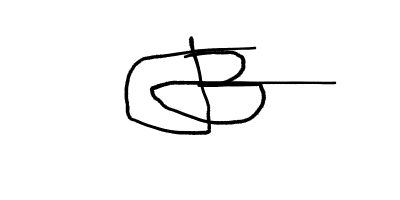
\includegraphics[height=1.4cm]{images/personal-signature.png}
    }\\
\end{tabularx}

\vspace{0pt plus1fill} %число перед fill = кратность относительно некоторого расстояния fill, кусками которого заполнены пустые места
\begin{center}
\textbf {\large \thesisAuthor}
\end{center}

\vspace{0pt plus3fill} %число перед fill = кратность относительно некоторого расстояния fill, кусками которого заполнены пустые места
\begin{center}
\textbf {\Large %\MakeUppercase
\thesisTitle}

\vspace{0pt plus3fill} %число перед fill = кратность относительно некоторого расстояния fill, кусками которого заполнены пустые места
{\large Специальность \thesisSpecialtyNumber\ "---\par <<\thesisSpecialtyTitle>>}

\ifdefined\thesisSpecialtyTwoNumber
{\large Специальность \thesisSpecialtyTwoNumber\ "---\par <<\thesisSpecialtyTwoTitle>>}
\fi

\vspace{0pt plus1.5fill} %число перед fill = кратность относительно некоторого расстояния fill, кусками которого заполнены пустые места
\Large{Автореферат}\par
\large{диссертации на соискание учёной степени\par \thesisDegree}
\end{center}

\vspace{0pt plus4fill} %число перед fill = кратность относительно некоторого расстояния fill, кусками которого заполнены пустые места
{\centering\thesisCity~--- \thesisYear\par}

\newpage
% оборотная сторона обложки
\thispagestyle{empty}
\noindent Работа выполнена в {\thesisInOrganization}.

\vspace{0.008\paperheight plus1fill}
\noindent%
\begin{tabularx}{\textwidth}{@{}lX@{}}
    \ifdefined\supervisorTwoFio
    Научные руководители:   & \supervisorRegalia\par
                              \ifdefined\supervisorDead
                              \framebox{\textbf{\supervisorFio}}
                              \else
                              \textbf{\supervisorFio}
                              \fi
                              \par
                              \vspace{0.013\paperheight}
                              \supervisorRegalia\par
                              \ifdefined\supervisorTwoDead
                              \framebox{\textbf{\supervisorTwoFio}}
                              \else
                              \textbf{\supervisorTwoFio}
                              \fi
                              \vspace{0.013\paperheight}\\
    \else
    Научный руководитель:   & \supervisorRegalia\par
                              \ifdefined\supervisorDead
                              \framebox{\textbf{\supervisorFio}}
                              \else
                              \textbf{\supervisorFio}
                              \fi
                              \vspace{0.013\paperheight}\\
    \fi
    Официальные оппоненты:  &
    \ifnumequal{\value{showopplead}}{0}{\vspace{13\onelineskip plus1fill}}{%
        \textbf{\opponentOneFio,}\par
        \opponentOneRegalia,\par
        \opponentOneJobPlace,\par
        \opponentOneJobPost\par
        \vspace{0.01\paperheight}
        \textbf{\opponentTwoFio,}\par
        \opponentTwoRegalia,\par
        \opponentTwoJobPlace,\par
        \opponentTwoJobPost
    \ifdefined\opponentThreeFio
        \par
        \vspace{0.01\paperheight}
        \textbf{\opponentThreeFio,}\par
        \opponentThreeRegalia,\par
        \opponentThreeJobPlace,\par
        \opponentThreeJobPost
    \fi
    }%
    \vspace{0.013\paperheight} \\
    \ifdefined\leadingOrganizationTitle
    Ведущая организация:    &
    \ifnumequal{\value{showopplead}}{0}{\vspace{6\onelineskip plus1fill}}{%
        \leadingOrganizationTitle
    }%
    \fi
\end{tabularx}
\vspace{0.008\paperheight plus1fill}

\noindent Защита состоится \defenseDate~на~заседании диссертационного совета \defenseCouncilNumber~при \defenseCouncilTitle~по адресу: \defenseCouncilAddress.

\vspace{0.008\paperheight plus1fill}
\noindent С диссертацией можно ознакомиться в библиотеке НИЯУ МИФИ.

\vspace{0.008\paperheight plus1fill}
\noindent Отзывы на автореферат в двух экземплярах, заверенные печатью учреждения, просьба направлять по адресу: \defenseCouncilAddress, ученому секретарю диссертационного совета~\defenseCouncilNumber.

\vspace{0.008\paperheight plus1fill}
\noindent{Автореферат разослан \synopsisDate.}

\noindent Телефон для справок: \defenseCouncilPhone.

\vspace{0.008\paperheight plus1fill}
\noindent%
\begin{tabularx}{\textwidth}{@{}%
>{\raggedright\arraybackslash}b{18em}@{}
>{\centering\arraybackslash}X
r
@{}}
    Ученый секретарь\par
    диссертационного совета\par
    \defenseCouncilNumber,\par
    \defenseSecretaryRegalia
    &
    \ifnumequal{\value{showsecrsign}}{0}{}{%
        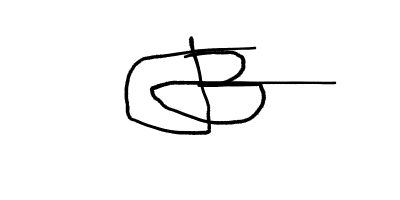
\includegraphics[width=2cm]{secretary-signature.png}%
    }%
    &
    \defenseSecretaryFio
\end{tabularx}
        % Титульный лист
%\mainmatter                   % В том числе начинает нумерацию страниц арабскими цифрами с единицы
\mainmatter*                  % Нумерация страниц не изменится, но начнётся с новой страницы
\section*{Общая характеристика работы}

\newcommand{\actuality}{\underline{\textbf{\actualityTXT}}}
\newcommand{\progress}{\underline{\textbf{\progressTXT}}}
\newcommand{\aim}{\underline{{\textbf\aimTXT}}}
\newcommand{\tasks}{\underline{\textbf{\tasksTXT}}}
\newcommand{\novelty}{\underline{\textbf{\noveltyTXT}}}
\newcommand{\influence}{\underline{\textbf{\influenceTXT}}}
\newcommand{\methods}{\underline{\textbf{\methodsTXT}}}
\newcommand{\defpositions}{\underline{\textbf{\defpositionsTXT}}}
\newcommand{\reliability}{\underline{\textbf{\reliabilityTXT}}}
\newcommand{\probation}{\underline{\textbf{\probationTXT}}}
\newcommand{\contribution}{\underline{\textbf{\contributionTXT}}}
\newcommand{\publications}{\underline{\textbf{\publicationsTXT}}}


{\actuality}
Построение ядерной энергетики нового типа, устойчивой к ресурсным ограничениям и предусматривающей решение проблемы обращения с радиоактивными отходами, связано с реакторами на быстрых нейтронах, обладающими размножающими свойствами. То есть, такая система, называемая двухкомпонентной ядерной энергетикой, нацелена на воспроизводство делящегося материала -- энергетического  плутония -- в реакторе на быстрых нейтронах. Однако, по оценкам \cite{andrianovaPERSPEKTIVNYETOPLIVNYEZAGRUZKI2015}, в ближайшие десятилетия, по мере становления двухкомпонентной ядерно-энергетической системы, неизбежен переходный период, когда делящиеся материалы будут повторно использоваться в топливном цикле реакторов на тепловых нейтронах, так как они составляют основную часть парка энергоблоков. Основным материалом топлива является уран, составляющий $\approx$95\% за вычетом конструкционных материалов. К тому же, оценки показывают, что регенерированный уран с содержанием $^{235}$U на уровне от $\approx$0,85\% экономически целесообразно дообогащать на изотопно-разделительном производстве \cite{NikipelovNikipelovSudby}. 

Итак, использование выделенного из отработавшего ядерного топлива (ОЯТ) регенерированного урана является основным достижимым в ближайшей перспективе направлением вовлечения регенерируемых материалов в топливный цикл энергетических реакторов. Выделенный из ОЯТ регенерированный уран может быть использован в составе топлива ВВЭР различными способами: центрифужное дообогащение для производства уранового топлива, дообогащение и включение в состав смешанного уран-плутониевого топлива типа REMIX.

Рецикл урана является сложной задачей ввиду присутствия в изотопном составе регенерата ряда четных изотопов. В первую очередь, это неприродные $^{232}$U и $^{236}$U. Присутствие первого затрудняет обращение с регенератом, как на стадии обогащения, так и на стадии производства твэлов. Влияние же второго сказывается на ухудшении размножающих свойств ядерного топлива, поскольку данный изотоп является паразитным поглотителем тепловых нейтронов. Вдобавок, в регенерате, по сравнению с природным ураном, на порядок выше содержание $^{234}$U При этом, ориентируясь на сегодняшние тенденции к увеличению длительности топливных циклов ВВЭР, которые связаны с повышением глубины выгорания топлива, следует принять во внимание вытекающий из этого рост содержания вредных четных изотопов в регенерате.

Итак, ввиду необходимости решения задачи эффективного вовлечения регенерированного урана в ядерный топливный цикл (ЯТЦ), существует потребность поиска и дальнейшей разработки каскадных схем, которые позволят решить задачу производства из регенерата свежего топлива, удовлетворяющего стандартным спецификациям.
На сегодняшний день, хоть и предложен ряд каскадов, которые могут быть полезны для этой задачи, их границы применимости могут быть недостаточны в условиях многократного рецикла.

Таким образом, учитывая принятое в ГК Росатом стратегическое решения перехода к замкнутому ЯТЦ, решение перечисленных задач представляется актуальным для современной разделительной науки. 

{\aim} диссертационной работы является изучение физических закономерностей
молекулярно-селективного массопереноса в ординарных и многопоточных каскадах
для разделения многокомпонентных смесей с целью дальнейшего поиска
оптимальных условий обогащения регенерированного урана в подобных каскадах при
его многократном использовании в различных видах регенерированного ядерного
топлива для реакторов на тепловых нейтронах.

Для~достижения поставленной цели необходимо было решить следующие {\tasks}:
\begin{enumerate}
  \item Анализ физических закономерностей массопереноса компонентов смеси
  регенерированного урана в ординарном каскаде.
  Выявление физических причин
  невозможности решения задачи обогащения регенерата произвольного изотопного
  состава в одиночном каскаде при одновременном выполнении условий на
  концентрации изотопов $^{232}$U, $^{234}$U и $^{236}$U в получаемом продукте – низкообогащенном уране, а также априорная оценка возможности или невозможности решения этой задачи.
  \item Физическое обоснование принципов построения двойных каскадов,
  позволяющих корректировать изотопный состав регенерата по концентрациям
  изотопов $^{232}$U, $^{234}$U и $^{236}$U с одновременным расходованием полного количества
  подлежащего обогащению регенерата при различных исходных концентрациях
  четных изотопов в нем.
  \item Обоснование физических принципов «утилизации» загрязненной четными
  изотопами фракции, возникающей в двойных каскадах, путем полной или
  частичной подачи данной фракции в третий каскад с предварительным
  перемешиванием ее с природным, обедненным и/или низкообогащенным ураном.
  \item Изучение физических закономерностей изменения изотопного состава регенерата и
  интегральных характеристик модифицированных двойных каскадов и тройных
  каскадов при обогащении регенерированного урана с различным исходным
  содержанием четных изотопов.
  \item Обобщение и систематизация подходов к выбору каскадной схемы, позволяющих
  эффективное обогащение регенерированного урана в условиях однократного и
  многократного рецикла.
  \item Определение физических закономерностей изменения изотопного состава
  регенерированного урана и параметров модифицированного двойного каскада для
  его дообогащения при многократном рецикле урана (отдельно и совместно с
  плутонием) в топливе реакторов типа ВВЭР.
\end{enumerate}


{\novelty}
\begin{enumerate}
  \item Впервые предложены модификации двойных каскадов, позволяющих корректировать
  изотопный состав регенерата по концентрациям изотопов $^{232}$U, $^{234}$U и $^{236}$U с одновременным расходованием полного количества подлежащего обогащению регенерата при различных исходных концентрациях четных изотопов в нем.
  \item Обоснованы физические принципы построения тройных каскадных схем для максимально полного использования использования исходного регенерированного урана для воспроизводства топлива реакторов на тепловых нейтронах.
  \item Выполнены оригинальные исследования по изучению физических закономерностей изменения изотопного состава регенерата и интегральных характеристик модифицированных двойных и тройных каскадах при обогащении регенерированного урана с различным исходным содержанием четных изотопов.
  \item Разработан обобщенный подход к выбору каскадной схемы для эффективного обогащения регенерированного урана в условиях однократного и многократного рецикла. Для этого были предложены критерии эффективности, такие как потери $^{235}$U в схеме и из регенерата, доля центрифуг, для которых превышается пороговое значение концентрации $^{232}$U, а также методы вычисления этих критериев в составных схемах.
  \item Развиты подходы оптимизации систем каскадов на основе двойного каскада: модифицированных двойных и тройных каскадов для обогащения регенерата урана по различным критериям
  эффективности, таким как:
  \begin{enumerate}
    \item расход природного урана
    \item затраты работы разделения
    \item доля потерь $^{235}$U в схеме
    \item доля потерь $^{235}$U из исходного регенерата
    \item доля ГЦ в схеме, в которых превышена предельно допустимая концентрация по $^{232}$U    
  \end{enumerate}
  \item Предложены пути утилизации высокоактивного «нештатного» отхода, образующегося в процессе обогащения регенерированного урана в двойном каскаде.
  \item Определены физические закономерности изменения изотопного состава регенерированного урана и параметров модифицированного двойного и тройного каскадов для его дообогащения при многократном рецикле урана (отдельно и совместно с плутонием) в топливе реакторов типа ВВЭР.
\end{enumerate}

{\influence} 
\begin{enumerate}
  \item Проведенный анализ физических закономерностей массопереноса компонентов смеси регенерированного урана в ординарном каскаде позволил однозначно определить условия при которых возможно/невозможно обогащение регенерированного урана различного исходного состава в одиночном каскаде.
  \item Разработанные модификации двойных и тройных каскадов позволяют эффективно решать задачу обогащения регенерированного урана с одновременным выполнением ограничений на концентрации четных изотопов и максимальным использованием исходного регенерата.
  \item Анализ результатов расчетного моделирования молекулярно-селективного массопереноса в модифицированных двойных и тройных каскадах для обогащения регенерата урана позволяет рекомендовать область практической применимости подобных схем для получения обогащенного регенерированного урана.
  \item Разработаны рекомендации по использованию результатов работы для обогащения регенерированного урана в условиях однократного и многократного рецикла в различных видах топлива.
  \item  Представленные в работе результаты могут быть использованы в расчетных группах на предприятиях и организациях, связанных как с проектированием и построением разделительных каскадов, так и непосредственным производством изотопной продукции (АО «Уральский электрохимический комбинат», АО «Сибирский химический комбинат», АО «ТВЭЛ», АО «Восточно-Европейский головной научно-исследовательский и проектный институт энергетических технологий», АО «ПО «ЭХЗ» и др.).
  \item Предложенные методики расчета могут лечь в основу технико-экономического анализа обращения с ОЯТ в части получения из восстановленного урана низкообогащенного урана, отвечающего требуемым качествам.  
  \item  Выводы работы применимы в рамках принятой ГК Росатом программы <<Сбалансированный ЯТЦ>>, нацеленной на обеспечение дополнительных конкурентных преимуществ направления зарубежных поставок ядерного топлива. Проводимое в данной работе исследование является перспективным для развития бизнеса ГК Росатом как в направлении топливных поставок, так и в обращении с облученным топливом \cite{efimenkoProblemyPerspektivyRazvitiya2017}.
  \item Разработан тренировочный программный комплекс для расчета каскада, нацеленного на возврат регенерированного урана. Код оформлен в виде лабораторной работы, которая затем внедрена в учебный процесс.
\end{enumerate}

{\methods}
Исследование проводит систематизацию научно-технической литературы, посвященной заявленной теме.
Применяются подходы, известные в современной теоретической физике, и в частности, в теории разделения изотопов в каскадах.
В ходе работы осуществляется обоснование теоретических принципов работы анализируемых каскадов, и математическое моделирование ранее не известных каскадных схем.
Для проведения расчетов использовались модельные каскады, а именно квазиидеальный каскад и его разновидность R-каскад, для которого принимается условие несмешивания пары выбранных компонентов. Рассматривался противоточный симметричный каскад ($\alpha=\beta=\sqrt{q}$).
Моделирование процессов разделения смесей изотопов урана проводилось с помощью специально разработанных специализированных компьютерных программ. Применялись современные программные средства языка программирования Julia и подключаемые библиотеки, такие как NLopt, Optim, предназначенные для решения систем нелинейных уравнений и нелинейной оптимизации, Plots.jl для визуализации результатов, и др..

{\defpositions}
\begin{enumerate}
  \item Результаты анализа физических закономерностей массопереноса компонентов смеси регенерированного урана в ординарном каскаде, позволяющие однозначно определить условия при которых возможно/невозможно обогащение регенерированного урана различного исходного состава в одиночном каскаде.
  \item Физико-математические модели, методики расчета и оптимизации модифицированных двойных и тройных каскадных схем для обогащения
  регенерата урана с одновременным выполнением условий на концентрации четных изотопов и максимальным использованием исходного материала.
  \item Методика выбора каскадной схемы обогащения регенерированного урана в условиях многократного рецикла, в зависимости от его исходного состава и принятых ограничений на концентрации четных изотопов.
\end{enumerate}
% В папке Documents можно ознакомиться в решением совета из Томского ГУ
% в~файле \verb+Def_positions.pdf+, где обоснованно даются рекомендации
% по~формулировкам защищаемых положений.

{\reliability} Надежность, достоверность и обоснованность научных положений и выводов, сделанных в диссертации, следует из корректности постановки задач, физической обоснованности применяемых приближений, использования в исследованиях методов, ранее примененных в аналогичных исследованиях, взаимной согласованности результатов исследования, а также из совпадения результатов численных экспериментов, полученных с помощью независимо разработанных методик как самим соискателем, так и другими исследователями. Корректность результатов вычислительных экспериментов гарантируется тестами и операторами проверки соответствия ограничениям, верифицирующими строгое выполнение заданных условий и соблюдение условий сходимости балансов (массовых и покомпонентных).

{\probation}
См. приложение А2.

{\contribution} Автор принимал активное участие в написании расчетных кодов, проведении вычислительных экспериментов, а также оформлении методики выбора каскадной схемы. Автором был разработан программный комплекс для сопровождения процесса принятия решений по выбору для заданной задачи каскада конфигурации, оптимальной по целевым критериям.

{\publications} 
См. приложение А1.



\section*{Содержание работы}
Во \underline{\textbf{введении}} обоснована актуальность разработки каскадных схем для обогащения регенерированного урана, вытекающая из задач долгосрочного устойчивого развития ядерной энергетики, а также из существующих на сегодня ограничений/недостатков ранее предложенных схем. Сформулирована цель исследования, состоящая в теоретическом обосновании эффективных способов обогащения регенерированного урана в каскадах центрифуг при его многократном использовании в регенерированном ядерном топливе для реакторов на тепловых нейтронах. Помимо этого, во \underline{\textbf{введении}} сформулированы научная новизна и практическая значимость выполненной работы, изложены основные положения, выносимые на защиту, обоснована достоверность полученных в работе результатов и представлены сведения об их апробации.

\underline{\textbf{Первая глава}} посвящена критическому анализу ранее предложенных каскадных схем обогащения регенерированного урана, а также краткому обзору источников по промышленному опыту обогащения регенерата урана. Проанализирована проблема четных изотопов $^{232,234,236}$U в задаче обогащения регенерированного урана с точки зрения разделительных технологий. Известно, что изотопы $^{232,234}$U ухудшают радиационные характеристики ядерного топлива (ЯТ), содержание $^{232}$U в НОУ-продукте ограничено мерами радиационной безопасности персонала на разделительном и фабрикационном производстве значениями $2\cdot10^{-7} \%$ или $5\cdot10^{-7} \%$, предельно допустимое отношение $\frac{C_{234,{P}}}{C_{235,{P}}} = 0,02$. Изотоп $^{236}$U вносит <<паразитный>> захват тепловых нейтронов в ЯТ, приводя к необходимости повышения его обогащения по $^{235}$U, что увеличивает затраты работы разделения в цикле. 

Описан процесс многократного использования (рецикла) урана в топливе реакторов на тепловых нейтронах (рис. \ref{fig_autoref1}) и подлежащие рассмотрению в диссертационной работе его стадии, а именно: обогащение регенерированного урана в каскадах центрифуг. Одним из факторов, осложняющих многократный рецикл урана является рост концентраций четных изотопов в процессе рецикла, что требует модификации известных каскадных схем, поскольку концентрации четных изотопов могут превышать допустимые пределы в несколько раз, что для примера проиллюстрировано взятыми из открытых источников составами регенерированного урана, прошедшего несколько рециклов (табл. \ref{is_compositions_2_5autoref}). Также при реализации схемы рис. \ref{fig_autoref1} подразумевают, что при производстве свежего топлива для реактора используют весь выделенный из ОЯТ этого же реактора регенерат, что проиллюстрировано на схеме рис. \ref{fig_autoref2}.  Такой подход призван обеспечить: (1) минимизацию потерь  $^{235}$U в топливном цикле; (2) максимально эффективно использовать потенциал ОЯТ для воспроизводства топлива; (3) исключить нежелательное накопление регенерата в процессе его многократного рецикла.
\begin{table}[h]
  \centering
  \caption{{Изотопные составы регенерата различных циклов{\label{is_compositions_2_5autoref}}}}
  \begin{tabular}{|c||c|c|c|c|c|c|}
  \hline Состав & Массовое число & 232 & 233 & 234 & 235 & 236 \\
  \hline 1 & C, \% & $6,62\cdot10^{-7}$ & $1,19\cdot10^{-6}$ & $3,28\cdot10^{-2}$ & 1,43 & 0,9932 \\
  2 & C, \% &  $1,03\cdot10^{-6}$ & $1,3\cdot10^{-6}$ & $3,91\cdot10^{-2}$ & 1,07 & 1,45 \\\hline
  \end{tabular}
\end{table}

\begin{figure}[ht]
  \centerfloat{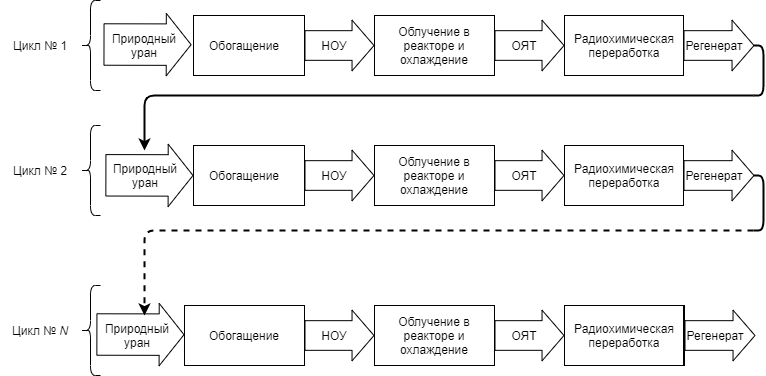
\includegraphics[scale=0.015]{cascades/recycling_ru}}
  \caption{Схема многократного рециклирования урана}\label{fig_autoref1}
\end{figure}

\begin{figure}[ht]
  \centerfloat{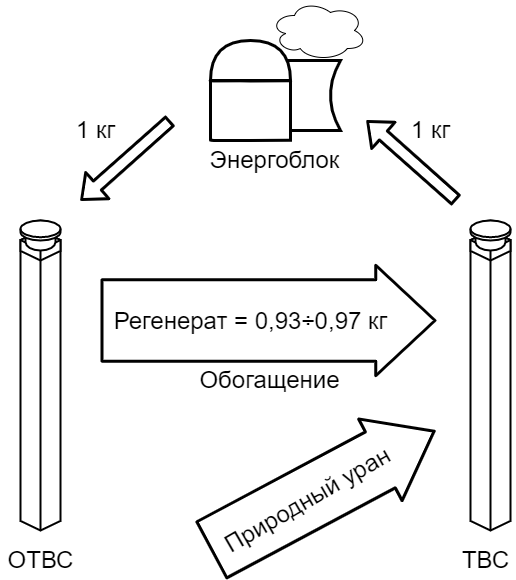
\includegraphics[scale=0.2]{cascades/ordinary/recycling1kg_ru}}
  \caption{Схема замыкания урановой топливной составляющей}\label{fig_autoref2}
\end{figure}

Приводится формулировка задачи обогащения регенерата, которой посвящена диссертационная работа: получение заданной массы товарного НОУ требуемого обогащения по $^{235}$U из заданной массы сырьевого регенерата урана (в том числе многократно рециклированного) с одновременным выполнением ограничений на концентрации четных изотопов. 

Показана невозможность использования ординарного (трехпоточного) каскада (рис. \ref{ordinary}) для решения сформулированной выше задачи в условиях многократного рецикла урана. Такой каскад можно использовать только для обогащения составов регенерата, в которых исходные концентрации четных изотопов меньше (на порядок или более), чем их допустимые пределы в товарном НОУ, что заведомо невыполнимо при многократном рецикле урана в современных реакторах на тепловых нейтронах (табл. \ref{is_compositions_2_5autoref}).

\begin{figure}[ht]
  \centerfloat{
\includegraphics[scale=0.025]{cascades/ordinary}}
  \caption{Схема ординарного трехпоточного каскада. Обозначения: $F$ --- поток питания; $P$ --- поток отбора; $W$ --- поток отвала}\label{ordinary}
\end{figure}

Анализ ранее предложенных способов обогащения регенерата позволяет условно разделить рассмотренные способы на 3 типа: (1) схемы с разбавлением четных изотопов; (2) схемы с отделением четных изотопов; (3) «гибридные» схемы (комбинируют первые два способа).
Показано, что лишь некоторые из известных способов потенциально могут решить поставленную задачу обогащения регенерата в условиях варьирования содержания четных изотопов в обогащаемом регенерате. Это делает необходимым дальнейший поиск каскадных схем для решения задачи, которые можно применять для различных исходных составов регенерированного урана, а также в случаях возможного изменения внешних условий задачи. 

\underline{\textbf{Во второй главе}} приведены основные понятия и определения теории разделения изотопов в каскадах. Введены понятия  разделительного элемента, разделительной ступени, разделительного каскада и возможных вариантов соединения ступеней в каскаде. Изложены основные сведения, необходимые для моделирования разделения многокомпонентных изотопных смесей в каскадах, описаны модели «квазиидеального» каскада, как частного случая симметричного противоточного каскада, и $R$-каскада. Рассмотрены основные варианты постановок задач расчета таких каскадов и алгоритмы их решения, которые будут использованы в 3-й и 4-й главах. 

\underline{\textbf{Третья глава}} посвящена анализу причин, затрудняющих или делающих невозможным использование описанных в главе 1 способов обогащения регенерата в условиях многократного рецикла. Рассмотрены различные варианты однокаскадных схем (рис. \ref{fig:diagram1ch3}), а также двойной каскад. В качестве схем на основе ординарного каскада рассмотрены:

\begin{enumerate}
  \item схема с разбавлением природным ураном предварительно обогащенного регенерата (рис. \ref{fig:diagram1ch3}.a);
  \item схема с разбавлением предварительно обогащенного регенерата низкообогащенным ураном (рис. \ref{fig:diagram1ch3}.b);
  \item схема с разбавлением предварительно обогащенного природного урана регенератом (рис. \ref{fig:diagram1ch3}.c);
  \item схема с разбавлением регенерата природным ураном перед подачей в ординарный трехпоточный каскад (рис. \ref{fig:diagram1ch3}.d).
\end{enumerate}

Для рассмотренных схем проведена серия вычислительных экспериментов, в которых варьировали параметры каждой из них при решении задачи обогащения регенерата, сформулированной выше. По результатам проведенных расчетов: (1) показана нецелесообразность использования схем на основе ординарных каскадов для обогащения регенерата в условиях многократного рецикла и невозможность решить задачу в большинстве случаев; (2) показана возможность обогащения регенерата с превышенными относительно допустимых пределов концентрациями четных изотопов в двойном каскаде. Однако двойной каскад позволяет только решить задачу, а именно обогатить регенерат по изотопу $^{235}$U и снизить концентрации четных изотопов, не решая, при этом, задачи полного использования регенерата. Другой проблема, связанной с использованием двойного каскада является высокое содержание $^{236}$U в получаемом НОУ-продукте (до 3\%), что приводит к необходимости повышения обогащения по $^{235}$U вплоть до 6-7\% и, соответственно, росту затрат работы разделения в топливном цикле на десятки процентов по сравнению с открытым ЯТЦ.

\begin{figure}[ht]
  \centerfloat{\includegraphics[scale=0.02]{cascades/ord_all}}
  \caption{Схемы обогащения регенерата на основе одиночного ординарного каскада. Обозначения: $E$ --- поток питающего схему регенерата, $F_n$ --- поток разбавителя (природного урана или низкообогащенного урана ($F_{leu}$)); $W$ --- поток отвального ОГФУ тяжелого конца каскада; $P$ --- товарный низкообогащенный уран}\label{fig:diagram1ch3}
\end{figure}

В главе также рассмотрен двойной каскад (рис. \ref{fig:double_ru_in3}), представляющий собой последовательное соединение двух каскадов, позволяющих сконцентрировать легкие четные изотопы отдельно от изотопа $^{235}$U. Для этого сначала в каскаде I обогащают изотоп $^{235}$U с одновременным обогащением изотопов $^{232}$U, $^{234}$U, $^{236}$U, а затем полученную смесь направляют на вход каскада II (рис. \ref{fig:double_ru_in3}), где она делится на две группы: в первой обогащены легкие изотопы ($^{232}$U, $^{234}$U и $^{235}$U), во второй обедняется $^{235}$U с более интенсивным обеднением $^{232}$U, $^{234}$U, что позволяет в потоке $W_2$ получить НОУ, отвечающий требованиям по концентрациям изотопов $^{232}$U, $^{234}$U с одновременной компенсацией $^{236}$U. Анализ проведенных расчетов обосновывает необходимость дальнейшего развития каскадных схем для решения задачи возврата регенерированного урана в ЯТЦ.

\begin{figure}[ht]
  \centerfloat{
\includegraphics[scale=0.055]{cascades/Double_core_pure}}
  \caption{Двойной каскад. Обозначения: $E$ --- поток питающего схему регенерата, $W_1$ --- поток отвального ОГФУ тяжелого конца каскада; $P$ ($W_2$) --- конечный НОУ продукт на основе регенерата; $P_2$ --- отход двойного каскада в виде высокообогащенного урана.}\label{fig:double_ru_in3}
\end{figure}


В \underline{\textbf{четвертой главе}} описаны предлагаемые в диссертации способы решения задачи обогащения регенерата в условиях его многократного рецикла.
В качестве базового предложенного способа рассмотрен <<двойной модифицированный каскад>> (рис. \ref{p2left_autoref}). Данный способ можно рассматривать в качестве развития способа, предложенного в патенте АО <<СХК>> №2282904 \cite{vodolazskihSposobIzotopnogoVosstanovleniya2006}. Идея работы предлагаемого в диссертационной работе способа состоит в следующем. В каскаде I обогащают исходный регенерат изотопами $^{232,233,234,235,236}$U. В каскаде II смесь делится на две фракции, так, чтобы в потоке тяжелой фракции ($W_2$) было понижено содержание $^{232,233,234}$U по отношению к питающей второй каскад смеси --- потоку $P_1$, при этом обогащение по $^{235}$U в потоке $W_2$ составляет величину несколько выше, чем требуется для товарного НОУ. Затем происходит разбавление потока $W_2$ смесью, не содержащей искусственных изотопов урана для выполнения ограничений по $^{232}$U и $^{236}$U, которая нарабатывается в каскаде III. В результате такого смешивания и получают финальный продукт --- товарный НОУ заданной массы и отвечающий всем требованиям по концентрациям четных изотопов. 

\begin{figure}[ht]
  \centerfloat{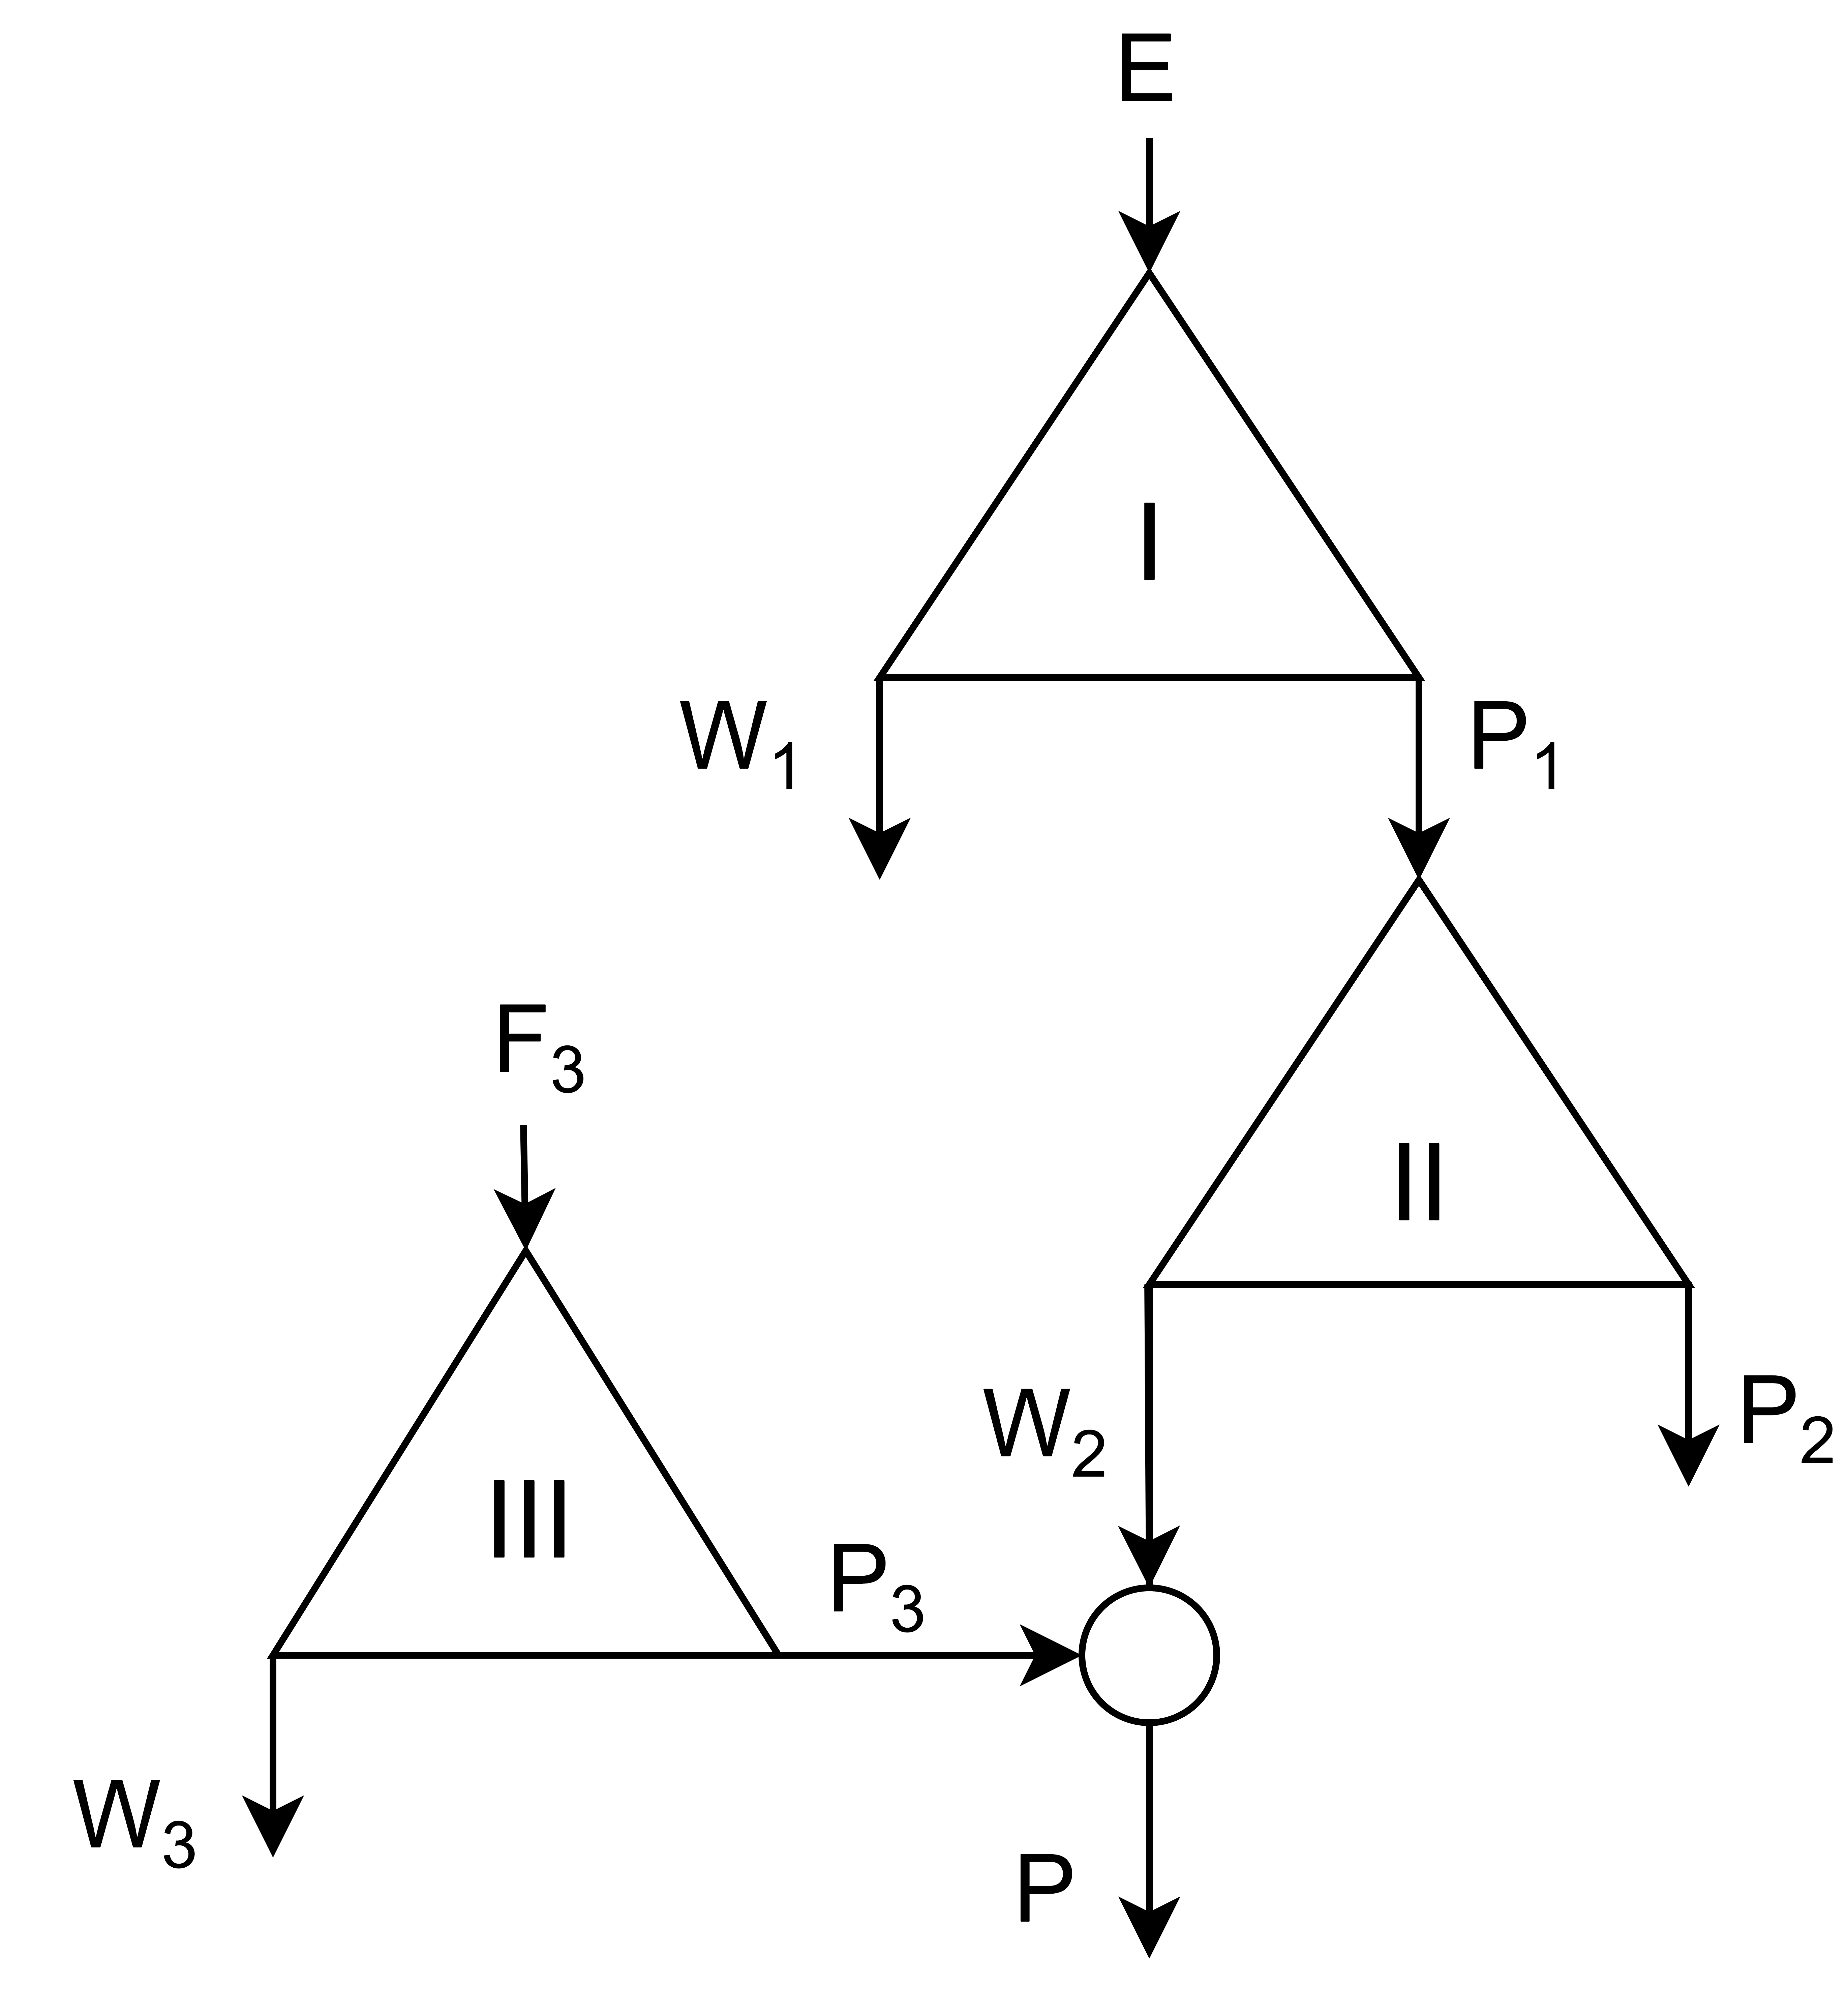
\includegraphics[scale=0.025]{cascades/DoubleModified23}}
  \caption{Схема модифицированного двойного каскада для обогащения регенерированного урана. Обозначения: $E$ --- поток регенерированного урана; $P_1$ --- поток отбора первого каскада, выступающий питанием второго каскада; $P_2$ --- поток отбора второго каскада; $W_1$ --- поток отвала первого каскада; $W_2$ --- поток тяжелой фракции (условный «отвал») второго каскада; $P_3$ --- поток НОУ-разбавителя на основе природного урана $F_3$; $P$ --- финальный продукт (товарный низкообогащенный уран (НОУ))}\label{p2left_autoref}
\end{figure}

Для каскадной схемы рис. \ref{p2left_autoref} в диссертационной работе предложена методика расчета и оптимизации ее параметров при решении задачи обогащения регенерата со всеми ограничениями. Предложенная методика основана на современных методах оптимизации функции многих переменных и может быть обобщена на случай оптимизации по различным критериям эффективности. Следует отметить, что предложенная методика оптимизации ранее не имеет аналогов в литературе, поскольку в ней впервые проведена оптимизация многокаскадной схемы как единой системы, в отличие от ранее использованных подходов с отдельной оптимизацией каждого из каскадов. С использованием разработанной методики оценена эффективность модифицированного двойного каскада при решении задачи обогащения урана в различных условиях и при оптимизации по таким критериям эффективности как:

\begin{enumerate}
  \item минимум расхода природного урана ($(\frac{\Delta A}{P})_\text{min}$);
  \item минимум затрат работы разделения ($(\frac{F_n}{P})_\text{min}$);
  \item максимум степени извлечения $^{235}$U в схеме ($(Y_f)_\text{max}$);
  \item максимум степени извлечения $^{235}$U из исходного регенерата ($(Y_{E})_\text{max}$).
\end{enumerate}  

В результате проведенных вычислительных экспериментов показано, что с использованием предложенной схемы даже для составов регенерированного урана с концентрациями четных изотопов выше предельных значений для товарного НОУ, возможно добиться экономии природного урана на уровне 15\% и выше при практически нулевом перерасходе или даже экономии затрат работы разделения. 

Проведено сравнение ранее предложенных каскадных схем и схемы рис. \ref{p2left_autoref} по ключевым характеристикам (расход природного урана, затраты работы разделения), во многом определяющим удельные затраты на товарный НОУ. Сравнение оптимальных параметров модифицированного двойного каскада с аналогичными характеристиками ранее известных способов обогащения регенерата показало преимущества предложенного способа по отношению к ним. Это выражается как в самом факте решения задачи, по отношению к способам, неспособным решить задачу, так и в лучших значениях расхода природного урана и затрат работы разделения по отношению к способам, решающим поставленную задачу. Результаты такого сравнения на примере обогащения регенерата состава 1 (табл. \ref{is_compositions_2_5autoref}) приведены в табл. \ref{allaut}. 

Для предложенного способа обогащения регенерата (рис. \ref{p2left_autoref}) проанализирована также его «устойчивость» к изменению внешних условий таких, как:
\begin{itemize}
  \item требуемое обогащение по изотопу $^{235}$U ($C_{235,P}$ от  4,4\% до  5,5\%);    
  \item величина предельно допустимой концентрации изотопа $^{232}$U в НОУ-продукте (варьировалась в интервале от $1\cdot10^{-7}$\% до $1\cdot10^{-6}$\%);
  \item расход регенерированного урана на единицу продукта ($E/P$ от 0,93 до 2,79).
\end{itemize}

Полученные результаты показали возможность решения задачи в широком диапазоне внешних условий, поскольку для всех рассмотренных комбинаций внешних параметров задачи были найдены решения, т.е. подобраны параметры модифицированного двойного каскада, обеспечившие решение задачи. Такие результаты показали, что схема применима как при текущих параметрах топливного цикла и требованиях к товарному НОУ, так и потенциально может быть применена при их изменении.

\begin{table}[ht]
  \centering
  \caption{Сравнение интегральных показателей (параметров П) схем для состава 1{\label{allaut}}}
  \begin{tabular}{|c|c|c|c|c|c|c|}
      \hline \diagbox{П}{Схема} & $\text{1}$ & $\text{2}$ & $\text{3}$ & $\text{4}$ & $\text{5}$ & $\text{6}$\\ \hline
      $\text{$Y_{f}$}$ & 78,9 & $5,3\cdot10^{-3}$ & 40,26 & 89,0 & 89,0 & 86,9\\ \hline
      $\text{$Y_{E}$}$ & 78,9 &  48,2 &              1,0 & ---    & 89,0 & 86,9\\ \hline
      $\text{$\delta(\frac{\Delta A}{P}), \%$}$ & 1,6 & 11,0 & $29,12$ & $11,0$ & 4,17 & $11,0$\\ \hline
      $\text{$\delta(\frac{F_n}{P}), \%$}$ & 21,1 & 15,2 & 12,86 & $17,0$ & 6,172 & $19,0$\\ \hline
      $\text{$\frac{P_{2}}{P}$}$ & $0$ & $0$ & $0$ & $0$ & $0$ & $0,0051$\\ \hline
      $\text{$\frac{E}{P}$}$ & $4,4$ & \hl{0,76} & \hl{0,6} & \hl{0,76} & 4,71 & $0,93$\\ \hline
      $\text{$C_{232,P}, \cdot10^{-7} \%$}$ & \hl{29,0} & 5,0 & 3,97 & 5,0 & 5,0 & 5,0\\ \hline
      $\frac{C_{234,P}}{C_{235,P}}$ & \hl{0,024} & $0,011$ & 0,01085 & $0,011$ & 0,0195 & $0,012$\\ \hline
      $\text{$C_{235,P}, \%$}$ & $5,95$ & $5,10$ & $5,12$ & $5,12$ & $6,0$ & $5,1$\\ \hline
      $\text{$C_{236,P}, \%$}$ & $3,4$ & $0,51$ & 0,596 & $0,6$ & $3,6$ & $0,68$\\ \hline
      \end{tabular}   
\end{table}

Отдельно проработаны способы дальнейшего использования (<<утилизации>>) загрязненной легкими изотопами $^{232,234}$U фракции (табл. \ref{P2_compositions_autoref}), получаемой в потоке $P_2$ двойного модифицированного каскада (рис. \ref{p2left_autoref}), которая в рассмотренном случае составляет 0,3\% от массы НОУ-продукта. Использование данной фракции призвано предотвратить нежелательное накопление на разделительном производстве высокоактивных отходов, а также задействовать остаточное содержание $^{235}$U в этом потоке, которое может достигать 20\% и более. Предложены следующие 3 способа: 

\begin{table}[h]
  \centering
  \caption{{Изотопный состав $P_2$.{\label{P2_compositions_autoref}}}}
    \begin{tabular}{|c|c|c|c|c|c|}
    \hline Массовое число & 232 & 233 & 234 & 235 & 236 \\
    \hline C, \% & $2,477\cdot10^{-5}$ & $5,438\cdot10^{-5}$ & 0,694 & 19,76 & 7,34 \\ \hline
  \end{tabular}
\end{table}

\begin{itemize}
  \item Перемешивание $P_2$ с регенератом, поступающим на обогащение (рис. \ref{P2utilizationRingautoref});
  \item Получение дополнительной массы товарного НОУ (рис. \ref{P2utilizationautoref});
  \item Перемешивание $P_2$ с обедненным ураном и последующее обогащение (рис. \ref{p2_withDepU}).
\end{itemize}

\begin{figure}[ht]
  \centerfloat{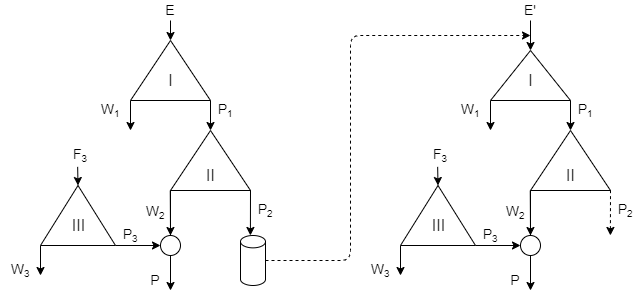
\includegraphics[scale=0.02]{cascades/P2utilizationRing}}
  \caption{Схема передачи загрязненного изотопом $^{232}$U состава гексафторида урана в двойном каскаде от первой партии дообогащенного регенерированного урана к последующей. Обозначения: $E$ --- поток регенерированного урана; $P_1$ --- поток отбора первого каскада, выступающий питанием второго каскада; $W_1$ --- поток отвала первого каскада; $W_2$ --- поток тяжелой фракции (условный «отвал») второго каскада; $P_3$ --- поток НОУ-разбавителя; $P$ --- финальный продукт (товарный низкообогащенный уран (НОУ)); $P_2$ --- поток отбора второго каскада, который подается на питание последующего двойного каскада, перемешиваясь с регенератом очередного рецикла}\label{P2utilizationRingautoref}
\end{figure}

\begin{figure}[ht]
  \centerfloat{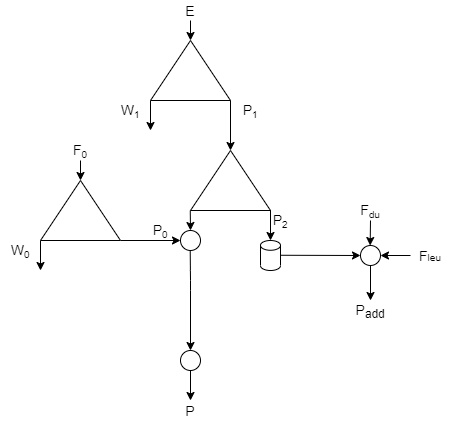
\includegraphics[scale=0.023]{cascades/P2utilization}}
  \caption{Схема независимого вовлечения в производство НОУ загрязненной изотопом $^{232}$U фракции, смешанной с обедненным и природным ураном}\label{P2utilizationautoref}
\end{figure}

Проведен сравнительный анализ предложенных вариантов <<утилизации>> загрязненной четными изотопа фракции. Каждый из рассмотренных способов вовлечения $P_2$ в ЯТЦ демонстрирует повышение эффективности использования $^{235}$U находящегося в регенерированном уране, что позволяет получить дополнительное увеличение экономии природного урана.

Для способа утилизации легкой фракции путем ее перемешивания с регенератом, поступающим на обогащение (рис. \ref{P2utilizationRingautoref}), проведены вычислительные эксперименты по топливоподготовке (обогащение регенерата с целью производства низкообогащенного урана) для серии частичных перегрузок топлива в реакторе (замена части ТВС активной зоны реактора)\footnote{формулировка задачи последовательного обогащения регенерата для нескольких перегрузок реактора со всеми условиями осуществлена совместно с сотрудниками НИЦ <<Курчатовский институт>>.}. Каждая из серий расчетов отличалась выбранным критерием эффективности, в качестве которых использованы $(Y_f)_\text{max}$, $(Y_{E})_\text{max}$, $(\delta(\frac{\Delta A}{P}))_\text{min}$, $(\delta(\frac{F_n}{P}))_\text{min}$, $(\frac{P_2}{P})_\text{min}$. По результатам анализа полученных закономерностей, с каждой последующей перегрузкой происходит снижение эффективности схемы по каждому из показателей.

Для способа независимого получения дополнительной массы товарного НОУ (рис. \ref{P2utilizationautoref}), была показана возможность получить экономию дополнительное количество природного урана относительно двойного модифицированного каскада.

Для оценки эффективности способа утилизации легкой фракции путем ее перемешивания с обедненным ураном и последующим обогащением, представленного на рис. \ref{p2_withDepU} разработаны методика и алгоритм расчета такой многокаскадной схемы. Предложенная методика обобщается на случай использования различных критериев эффективности. Проведенные с ее помощью серии вычислительных экспериментов показывают возможность обеспечить экономию природного урана и затрат работы разделения по отношению к открытому ЯТЦ даже в случае обогащения регенерата с высоким содержанием $^{232}$U (выше предельных значений для товарного НОУ).

\begin{figure}[ht]
  \centerfloat{\includegraphics[scale=0.02]{cascades/triple_cascade23}}
  \caption{Тройной каскад для обогащения регенерированного урана. Обозначения: $E$ --- поток регенерированного урана; $P_1$ --- поток отбора первого каскада, выступающий питанием второго каскада; $P_2$ --- поток отбора второго каскада; $F_{D}$ --- поток ОГФУ-разбавителя, смешиваемого с $P_2$ перед подачей на вход третьего каскада; $W_1$ --- поток отвала первого каскада; $W_2$ --- поток тяжелой фракции (условный «отвал») второго каскада; $P_3$ --- поток НОУ-разбавителя на основе природного урана $F_3$; $P$ --- финальный продукт (товарный низкообогащенный уран (НОУ)), полученный смешиванием потоков $W_2$, $P_3$ и $P_4$, где $P_4$ --- отбор третьего каскада; $W_4$ --- отвал третьего каскада}\label{p2_withDepU}
\end{figure}

По результатам исследования схем, представляющих собой различные способы утилизации побочной фракции $P_2$, представлена сравнительная таблица \ref{3loopautoref}.
\begin{table}
  \centering
  \caption{Сравнение интегральных показателей способов утилизации загрязненного продукта для состава 1. Обозначения: П --- параметр, ср. --- среднее, сп. --- способ{\label{3loopautoref}}}
  \renewcommand{\arraystretch}{1.2}
  \begin{tabular}{|r|c|c|c|c|c|c|c|c|c|}
    \hline
    \multirow{2}{*}{П} & \multicolumn{3}{c|}{сп. 1} & \multicolumn{3}{c|}{сп. 2} & \multicolumn{3}{c|}{сп. 3}\\
    \cline{2-10}
    & {\tiny Загр.} 1 & {\tiny Загр.} 2 & ср. & {\tiny Загр.} 1 & {\tiny Загр.} 2 & ср. & {\tiny Загр.} 1 & {\tiny Загр.} 2 & ср. \\
    \hline
    $\frac{F_n}{P}$   & 6,40 & 6,49 & 6,45    & 6,40  & 6,40  & 6,40    & 6,23 & 6,23 & 6,23\\ \hline
    $\frac{\Delta A}{P}, \textit{{\tiny ЕРР}}$ & 11,26 & 11,61 & 11,43 & 11,26 & 11,29 & 11,27   & 11,66 & 11,66 & 11,66 \\ \hline
    $\frac{P_2}{P}, \%$  & 0,49 & 2,96 & 1,73    & 0,49 & 0,91 & 0,7        & 0 & 0 & 0 \\ \hline
    $\frac{E}{P}$        & 0,93 & 0,95 & 0,94    & 0,93 & 1,08 & 1,01     & 0,93 & 0,93 & 0,93 \\ \hline
  \end{tabular}
\end{table}

Как следует из анализа данных табл. \ref{3loopautoref}, использование схемы независимой утилизации $P_2$ (сп. 2, представленная на рис. \ref{P2utilizationautoref}) для формирования Загр. 2, позволяет, по сравнению со схемой с замыканием (сп. 1, Загр. 2, рис. \ref{P2utilizationRingautoref}), расходовать меньшее удельное количество природного урана и работы разделения (на $\approx$1,3\% и $\approx$2,7\%) на этапе производства НОУ-продукта для осуществления перегрузки топлива в реакторе, и снижать количество отхода в виде $P_2$ в более чем три раза. То есть, схема независимой утилизации $P_2$ показывает лучшие результаты по ключевым (интегральным) показателям, по сравнению со схемой модифицированного двойного каскада.

Способ 3 (тройной каскад) позволяет задействовать все требуемое количество регенерата на каждой перегрузке, а также позволяет добиться наименьшего расхода природного урана, обеспечивая $\approx$4\% выигрыша, по сравнению со способом 1 на этапе производства урана для Загр. 2, при этом перерасходуя работу разделения лишь на $\approx$0,5\% и не производя побочного отхода с высоким содержанием $^{232,234}$U, такого как $P_2$.

\newpage

\pdfbookmark{Заключение}{conclusion}
В \underline{\textbf{заключении}} перечислены полученные ключевые результаты диссертационного исследования и сформулированы его основные выводы.

Теоретически обоснованы способы обогащения регенерированного урана с одновременной коррекцией его изотопного состава по содержанию четных изотопов, основанных на модификациях двойных каскадов. Показана применимость предложенных модификаций двойного каскада в условиях обогащения регенерированного урана с исходным содержанием четных изотопов выше допустимых пределов, что в несколько раз превышает содержание указанных изотопов в составах регенерата ранее рассмотренных в теоретических исследованиях. Это означает возможность успешного использования предложенных подходов в условиях многократного рецикла, когда концентрации четных изотопов возрастают от рецикла к рециклу.

По результатам проведенного исследования можно сформулировать следующие конкретные выводы.

\begin{enumerate}
\item В работе предложена модификация двойного каскада с НОУ-разбавителем из природного урана, применимая для обогащения регенерированного урана в условиях многократного рецикла урана в топливе легководных реакторов и позволяющая получить продукт, отвечающий всем требованиям на концентрации четных изотопов для регенерата различного исходного состава. Достоинствами схемы является возможность частичного отделения легких изотопов $^{232}$U, $^{234}$U от $^{235}$U, а также обособленность участков обогащения регенерированного урана и природного урана. Последнее обеспечивает большую вариативность в возможностях практической реализации подобной схемы, а также позволяет избежать загрязнения значительной части разделительного оборудования четными изотопами урана.


Процесс обогащения регенерата урана различного исходного состава в предложенной схеме смоделирован с использованием теории квазиидеального каскада. Разработаны оригинальные методики расчета и оптимизации предложенной каскадной схемы по различным критериям эффективности, таким как минимум расхода природного урана, минимум затрат работы разделения на получение конечного продукта, максимум степени извлечения целевого изотопа $^{235}$U из исходного регенерата и др. Проведена серия вычислительных экспериментов, позволившая оценить ключевые интегральные характеристики предложенной модификации двойного каскада (удельный расход природного урана, затраты работы разделения) в широком диапазоне изменение как ее параметров, так и внешних условий. Анализ результатов проведенных вычислительных экспериментов показал, что схема оказывается устойчивой в случаях, когда внешние ограничения <<ужесточаются>>. Например, уменьшается предельно допустимая концентрация $^{232}$U в товарном НОУ или кратно (до трех раз) возрастает масса исходного регенерированного урана, которую нужно израсходовать для получения заданной массы товарного продукта. Анализ полученных результатов создает базис для дальнейшей практической реализации подобной схемы и поиска наиболее эффективных режимов ее работы.

Анализ эффективности предложенной каскадной схемы с точки зрения потерь $^{235}$U показал, что схема позволяет извлечь более 85\% от массы $^{235}$U из исходного регенерированного урана, поступившего на обогащение. Это обеспечивает экономию природного урана по сравнению с открытым топливным циклом на уровне 15-20\% в зависимости от исходного изотопного состава регенерата. Таким образом, эта схема превышает аналогичные показатели для простейших разбавляющих схем практически вдвое.
\item Обоснован способ эффективной «утилизации» загрязненной четными изотопами фракции, возникающей в двойных каскадах при очистке от $^{232}$U, с учетом полной или частичной подачи данной фракции: а) в третий каскад с предварительным перемешиванием ее с природным, обедненным и/или низкообогащенным ураном; б) в отдельный двойной каскад, осуществляющий наработку низкообогащенного урана для последующей топливной кампании реактора. Для каждого из предложенных способов проведены вычислительные эксперименты, анализ результатов которых позволил сформулировать достоинства и недостатки каждого из способов и очертить возможные области их применения.
В качестве основных выводов по этой части приведем следующие:
\begin{enumerate}
\item Характерными недостатками схемы двойного каскада с НОУ-разбавителем с возвратом потока загрязненной $^{232}$U фракции в цикл является возврат значительной части четных изотопов на вход каскадной схемы. Это приводит к тому, что при повторении такого процесса несколько раз концентрации четных изотопов в исходном регенерате могут существенно возрастать (до нескольких раз), тем самым снижая эффективность обогащения регенерата в целом. Следовательно, такой подход применим для 1-3 таких возвратов, далее целесообразно рассмотреть возможность реализации одного из других предложенных способов утилизации отхода.
\item Характерным недостатком схемы тройного каскада для утилизации загрязненной $^{232}$U фракции является увеличение затрат работы разделения по отношению к другим рассмотренным модификациям, возникающее при обогащении разбавленного обедненным ураном загрязненного четными изотопами отхода. Анализ результатов серии вычислительных экспериментов, проведенных для данной схемы позволяет говорить, что она хорошо применима для составов регенерированного урана, когда исходное содержание $^{232}$U еще не превысило предельно допустимых значений для продукта. Иными словами, такой подход может подойти для обогащения регенерата 1-го и 2-го рецикла, позволяя вернуть в цикл более 90\% массы $^{235}$U из регенерированного урана. 
\item Схема утилизации загрязненной $^{232}$U фракции через ее разбавление обедненным ураном и НОУ из природного урана обеспечивает возможность наработки дополнительной массы отвечающего всем требованиям товарного продукта. При этом в схеме отсутствуют дополнительные каскады, что исключает дополнительные затраты работы разделения. Показано, что данный способ утилизации пригоден при обогащении различных вариантов составов исходного регенерата, что делает его перспективным в условиях многократного рецикла.
\end{enumerate}

\item Результаты работы дают основу для проведения дальнейшего технико-экономического анализа каждой из схем на основе их интегральных показателей, таких как расход природного урана, затраты работы разделения, потери $^{235}$U в цикле в контексте всей цепочки ядерного топливного цикла, а также с учетом возникающих в этой цепочке изменений при использовании регенерата урана по отношению к открытому топливному циклу. Помимо этого, необходима проработка технологических проблем каждой из схем, в частности, с точки зрения возможности эксплуатации и обслуживания оборудования в условиях работы с материалами, имеющими более высокую, чем природный уран удельную активность. 
\end{enumerate}


\insertbibliofull   
\pdfbookmark{Литература}{bibliography}













































% \ifdefmacro{\microtypesetup}{\microtypesetup{protrusion=false}}{} % не рекомендуется применять пакет микротипографики к автоматически генерируемому списку литературы
% \urlstyle{rm}                               % ссылки URL обычным шрифтом
% \ifnumequal{\value{bibliosel}}{0}{% Встроенная реализация с загрузкой файла через движок bibtex8
%     \renewcommand{\bibname}{\large \bibtitleauthor}
%     \nocite{*}
%     \insertbiblioauthor           % Подключаем Bib-базы
%     %\insertbiblioexternal   % !!! bibtex не умеет работать с несколькими библиографиями !!!
% }{% Реализация пакетом biblatex через движок biber
%     % Цитирования.
%     %  * Порядок перечисления определяет порядок в библиографии (только внутри подраздела, если `\insertbiblioauthorgrouped`).
%     %  * Если не соблюдать порядок "как для \printbibliography", нумерация в `\insertbiblioauthor` будет кривой.
%     %  * Если цитировать каждый источник отдельной командой --- найти некоторые ошибки будет проще.
%     %
%     %% authorvak
%     \nocite{smirnovObogashchenieRegenerirovannogoUrana2018}%
%     % \nocite{vakbib2}%
%     % %
%     % %% authorwos
%     % \nocite{wosbib1}%
%     % %
%     % %% authorscopus
%     % \nocite{smirnovApplyingEnrichmentCapacities2018}%
%     % %
%     % %% authorpathent
%     % \nocite{patbib1}%
%     % %
%     % %% authorprogram
%     % \nocite{progbib1}%
%     % %
%     % %% authorconf
%     \nocite{smirnovApplyingEnrichmentCapacities2018}%
%     % \nocite{confbib2}%
%     % %
%     % %% authorother
%     % \nocite{bib1}%
%     % \nocite{bib2}%

%     \ifnumgreater{\value{usefootcite}}{0}{
%         \begin{refcontext}[labelprefix={}]
%             \ifnum \value{bibgrouped}>0
%                 \insertbiblioauthorgrouped    % Вывод всех работ автора, сгруппированных по источникам
%             \else
%                 \insertbiblioauthor      % Вывод всех работ автора
%             \fi
%         \end{refcontext}
%     }{
%         \ifnum \totvalue{citeexternal}>0
%             \begin{refcontext}[labelprefix=A]
%                 \ifnum \value{bibgrouped}>0
%                     \insertbiblioauthorgrouped    % Вывод всех работ автора, сгруппированных по источникам
%                 \else
%                     \insertbiblioauthor      % Вывод всех работ автора
%                 \fi
%             \end{refcontext}
%         \else
%             \ifnum \value{bibgrouped}>0
%                 \insertbiblioauthorgrouped    % Вывод всех работ автора, сгруппированных по источникам
%             \else
%                 \insertbiblioauthor      % Вывод всех работ автора
%             \fi
%         \fi
%         %  \insertbiblioauthorimportant  % Вывод наиболее значимых работ автора (определяется в файле characteristic во второй section)
%         \begin{refcontext}[labelprefix={}]
%             \insertbibliofull            % Вывод списка литературы, на которую ссылались в тексте автореферата
%         \end{refcontext}
%         % Невидимый библиографический список для подсчета количества внешних публикаций
%         % Используется, чтобы убрать приставку "А" у работ автора, если в автореферате нет
%         % цитирований внешних источников.
%         \printbibliography[heading=nobibheading, section=0, env=countexternal, keyword=biblioexternal, resetnumbers=true]%
%     }
% }
% \ifdefmacro{\microtypesetup}{\microtypesetup{protrusion=true}}{}
% \urlstyle{tt} 
      % Содержание автореферата


\appendix
\section*{Список публикаций автора}
\begin{refsection}   
    \cite{nevinicaToplivnyyCiklLegkovodnogo2019, smirnovObogashchenieRegenerirovannogoUrana2018,
    smirnovApplyingEnrichmentCapacities2018,
    rodionovaAnalizTehnikoekonomicheskihHarakteristik2019,
    smirnovMethodEnrichReprocessed2019,
    smirnovFizikotehnicheskieProblemyObogashcheniya2020,
    gusevMultycascadeEnrichmentSchemes2020,
    gusevProliferationResistanceAnalysis2019,
    smirnovInfluenceUncertaintiesIsotopic2017,
    gusevFeaturesLightwaterReactor2018}
\printbibliography[heading=subbibliography]
\end{refsection}


%%% Выходные сведения типографии
\newpage\thispagestyle{empty}

\vspace*{0pt plus1fill}

\small
\begin{center}
    \textit{\thesisAuthor}
    \par\medskip

    \thesisTitle
    \par\medskip

    Автореф. дис. на соискание ученой степени \thesisDegreeShort
    \par\bigskip

    Подписано в печать \blank[\widthof{999}].\blank[\widthof{999}].\blank[\widthof{99999}].
    Заказ № \blank[\widthof{999999999999}]

    Формат 60\(\times\)90/16. Усл. печ. л. 1. Тираж 13 экз.
    %Это не совсем формат А5, но наиболее близкий, подробнее: http://ru.wikipedia.org/w/index.php?oldid=78976454

    Типография \blank[0.5\linewidth]
\end{center}
\cleardoublepage

\end{document}
